\documentclass[]{book}
\usepackage{lmodern}
\usepackage{amssymb,amsmath}
\usepackage{ifxetex,ifluatex}
\usepackage{fixltx2e} % provides \textsubscript
\ifnum 0\ifxetex 1\fi\ifluatex 1\fi=0 % if pdftex
  \usepackage[T1]{fontenc}
  \usepackage[utf8]{inputenc}
\else % if luatex or xelatex
  \ifxetex
    \usepackage{mathspec}
  \else
    \usepackage{fontspec}
  \fi
  \defaultfontfeatures{Ligatures=TeX,Scale=MatchLowercase}
\fi
% use upquote if available, for straight quotes in verbatim environments
\IfFileExists{upquote.sty}{\usepackage{upquote}}{}
% use microtype if available
\IfFileExists{microtype.sty}{%
\usepackage{microtype}
\UseMicrotypeSet[protrusion]{basicmath} % disable protrusion for tt fonts
}{}
\usepackage[margin=1.5in]{geometry}
\usepackage{hyperref}
\hypersetup{unicode=true,
            pdftitle={Package Development in R},
            pdfborder={0 0 0},
            breaklinks=true}
\urlstyle{same}  % don't use monospace font for urls
\usepackage{natbib}
\bibliographystyle{apalike}
\usepackage{color}
\usepackage{fancyvrb}
\newcommand{\VerbBar}{|}
\newcommand{\VERB}{\Verb[commandchars=\\\{\}]}
\DefineVerbatimEnvironment{Highlighting}{Verbatim}{commandchars=\\\{\}}
% Add ',fontsize=\small' for more characters per line
\usepackage{framed}
\definecolor{shadecolor}{RGB}{248,248,248}
\newenvironment{Shaded}{\begin{snugshade}}{\end{snugshade}}
\newcommand{\KeywordTok}[1]{\textcolor[rgb]{0.13,0.29,0.53}{\textbf{#1}}}
\newcommand{\DataTypeTok}[1]{\textcolor[rgb]{0.13,0.29,0.53}{#1}}
\newcommand{\DecValTok}[1]{\textcolor[rgb]{0.00,0.00,0.81}{#1}}
\newcommand{\BaseNTok}[1]{\textcolor[rgb]{0.00,0.00,0.81}{#1}}
\newcommand{\FloatTok}[1]{\textcolor[rgb]{0.00,0.00,0.81}{#1}}
\newcommand{\ConstantTok}[1]{\textcolor[rgb]{0.00,0.00,0.00}{#1}}
\newcommand{\CharTok}[1]{\textcolor[rgb]{0.31,0.60,0.02}{#1}}
\newcommand{\SpecialCharTok}[1]{\textcolor[rgb]{0.00,0.00,0.00}{#1}}
\newcommand{\StringTok}[1]{\textcolor[rgb]{0.31,0.60,0.02}{#1}}
\newcommand{\VerbatimStringTok}[1]{\textcolor[rgb]{0.31,0.60,0.02}{#1}}
\newcommand{\SpecialStringTok}[1]{\textcolor[rgb]{0.31,0.60,0.02}{#1}}
\newcommand{\ImportTok}[1]{#1}
\newcommand{\CommentTok}[1]{\textcolor[rgb]{0.56,0.35,0.01}{\textit{#1}}}
\newcommand{\DocumentationTok}[1]{\textcolor[rgb]{0.56,0.35,0.01}{\textbf{\textit{#1}}}}
\newcommand{\AnnotationTok}[1]{\textcolor[rgb]{0.56,0.35,0.01}{\textbf{\textit{#1}}}}
\newcommand{\CommentVarTok}[1]{\textcolor[rgb]{0.56,0.35,0.01}{\textbf{\textit{#1}}}}
\newcommand{\OtherTok}[1]{\textcolor[rgb]{0.56,0.35,0.01}{#1}}
\newcommand{\FunctionTok}[1]{\textcolor[rgb]{0.00,0.00,0.00}{#1}}
\newcommand{\VariableTok}[1]{\textcolor[rgb]{0.00,0.00,0.00}{#1}}
\newcommand{\ControlFlowTok}[1]{\textcolor[rgb]{0.13,0.29,0.53}{\textbf{#1}}}
\newcommand{\OperatorTok}[1]{\textcolor[rgb]{0.81,0.36,0.00}{\textbf{#1}}}
\newcommand{\BuiltInTok}[1]{#1}
\newcommand{\ExtensionTok}[1]{#1}
\newcommand{\PreprocessorTok}[1]{\textcolor[rgb]{0.56,0.35,0.01}{\textit{#1}}}
\newcommand{\AttributeTok}[1]{\textcolor[rgb]{0.77,0.63,0.00}{#1}}
\newcommand{\RegionMarkerTok}[1]{#1}
\newcommand{\InformationTok}[1]{\textcolor[rgb]{0.56,0.35,0.01}{\textbf{\textit{#1}}}}
\newcommand{\WarningTok}[1]{\textcolor[rgb]{0.56,0.35,0.01}{\textbf{\textit{#1}}}}
\newcommand{\AlertTok}[1]{\textcolor[rgb]{0.94,0.16,0.16}{#1}}
\newcommand{\ErrorTok}[1]{\textcolor[rgb]{0.64,0.00,0.00}{\textbf{#1}}}
\newcommand{\NormalTok}[1]{#1}
\usepackage{longtable,booktabs}
\usepackage{graphicx,grffile}
\makeatletter
\def\maxwidth{\ifdim\Gin@nat@width>\linewidth\linewidth\else\Gin@nat@width\fi}
\def\maxheight{\ifdim\Gin@nat@height>\textheight\textheight\else\Gin@nat@height\fi}
\makeatother
% Scale images if necessary, so that they will not overflow the page
% margins by default, and it is still possible to overwrite the defaults
% using explicit options in \includegraphics[width, height, ...]{}
\setkeys{Gin}{width=\maxwidth,height=\maxheight,keepaspectratio}
\IfFileExists{parskip.sty}{%
\usepackage{parskip}
}{% else
\setlength{\parindent}{0pt}
\setlength{\parskip}{6pt plus 2pt minus 1pt}
}
\setlength{\emergencystretch}{3em}  % prevent overfull lines
\providecommand{\tightlist}{%
  \setlength{\itemsep}{0pt}\setlength{\parskip}{0pt}}
\setcounter{secnumdepth}{5}
% Redefines (sub)paragraphs to behave more like sections
\ifx\paragraph\undefined\else
\let\oldparagraph\paragraph
\renewcommand{\paragraph}[1]{\oldparagraph{#1}\mbox{}}
\fi
\ifx\subparagraph\undefined\else
\let\oldsubparagraph\subparagraph
\renewcommand{\subparagraph}[1]{\oldsubparagraph{#1}\mbox{}}
\fi

%%% Use protect on footnotes to avoid problems with footnotes in titles
\let\rmarkdownfootnote\footnote%
\def\footnote{\protect\rmarkdownfootnote}

%%% Change title format to be more compact
\usepackage{titling}

% Create subtitle command for use in maketitle
\providecommand{\subtitle}[1]{
  \posttitle{
    \begin{center}\large#1\end{center}
    }
}

\setlength{\droptitle}{-2em}

  \title{Package Development in R}
    \pretitle{\vspace{\droptitle}\centering\huge}
  \posttitle{\par}
    \author{}
    \preauthor{}\postauthor{}
      \predate{\centering\large\emph}
  \postdate{\par}
    \date{August 2019}

\usepackage{booktabs}

\usepackage{epsfig}
\usepackage{epstopdf}
\usepackage{rotate}
\usepackage{graphicx}
\usepackage{hyperref}
\usepackage{alphalph}
\usepackage{caption}
\usepackage[hang,flushmargin]{footmisc}
\usepackage{framed}
\usepackage{xcolor}
\usepackage{verbatim} 

\usepackage{bm}
\setcounter{MaxMatrixCols}{20}
\newcommand{\Var}{\mathrm{Var}}
\newcommand{\SD}{\mathrm{SD}}
\newcommand{\Cov}{\mathrm{Cov}}
\newcommand{\fx}{f({\bf x})}
\newcommand\R{{\textsf R~}}
\newcommand\Rst{\textsf{RStudio}}

% spacing between environments
\usepackage{amsthm}
\makeatletter
\def\thm@space@setup{%
  \thm@preskip=15pt plus 2pt minus 4pt
  \thm@postskip=\thm@preskip
}
\makeatother


% Title format
\usepackage{titling}
\pretitle{\Huge\sffamily}
\posttitle{\par\vskip 0.5em}
\predate{\LARGE\sffamily}
\postdate{\par}

\urlstyle{tt}

\begin{document}
\maketitle

{
\setcounter{tocdepth}{1}
\tableofcontents
}
\chapter*{Introduction}\label{introduction}
\addcontentsline{toc}{chapter}{Introduction}

\section*{Table of Contents}\label{table-of-contents}
\addcontentsline{toc}{section}{Table of Contents}

This guide is organized into three parts.

\begin{enumerate}
\def\labelenumi{\arabic{enumi}.}
\tightlist
\item
  First, we'll run through \href{./package-development.html}{The proper
  way to structure and test packages}.
\item
  Second, we'll discuss \href{./version-control.html}{Version Control
  with Git and GitHub}
\item
  Lastly, we'll
  \href{./integrated-development-environments.html}{briefly look at a
  couple of IDEs}, which are just pieces of software that make it easier
  to write packages.
\end{enumerate}

\href{https://www.rstudio.com/wp-content/uploads/2015/03/devtools-cheatsheet.pdf}{Here's
a link to a great devtools cheatsheet} which puts most of the useful
commands in this guide in one place.

We also wrote a small development example package (called
\texttt{devex}) which you can find linked
\href{https://github.com/IQSS/dss-rbuild/tree/master/devex}{here, on
GitHub}. If you haven't used GitHub yet, don't worry - we'll go over how
to use GitHub later.

Also, this guide is still under development, and we take feedback! If
you find anything confusing or think the guide misses important content,
please email
\href{mailto:help@iq.harvard.edu}{\nolinkurl{help@iq.harvard.edu}}

\section*{Authors and Sources}\label{authors-and-sources}
\addcontentsline{toc}{section}{Authors and Sources}

It's worth acknowledging a few people who helped make this guide
possible. First of all, Simo Goshev and Steve Worthington at Harvard's
IQSS helped design the structure of the guide and edited the content.
Second, Asher Spector at Harvard College did the hard work of actually
writing the tutorial in Rmarkdown and configuring the GitHub repo and
website. Third, Jinjie Liu at IQSS helped to polish the content. Fourth,
this guide was written for a different audience, but a lot of its
structure and content is based on Hadley Wickham's book
\href{http://r-pkgs.had.co.nz/}{R Packages}. To help write the sections
on testing, we also referenced
\href{http://slides.com/christophergandrud/failing-faster\#/24}{Christopher
Gandrud's `Failing Faster' Presentation}, and
\href{https://github.com/IQSS/social_science_software_toolkit/blob/master/testing/recommended_testing_tools_R.md\#recommended-testing-tools-and-process-for-r-packages}{Christopher
Gandrud's Broader Testing Guidelines}. For the section on on Version
Control, we referenced \href{https://kbroman.org/github_tutorial/}{Karl
Broman's Book}, a
\href{https://www.git-tower.com/learn/git/faq/restore-repo-to-previous-revision}{Git-Tower
post}, and the GitHub documentation
\href{https://git-scm.com/book/en/v2/Getting-Started-Git-Basics}{here}
and
\href{https://git-scm.com/book/en/v2/Getting-Started-First-Time-Git-Setup}{here}
to help write this guide.

\chapter{Package Development}\label{package-development}

The following graphic outlines this entire chapter:

\begin{figure}
\centering
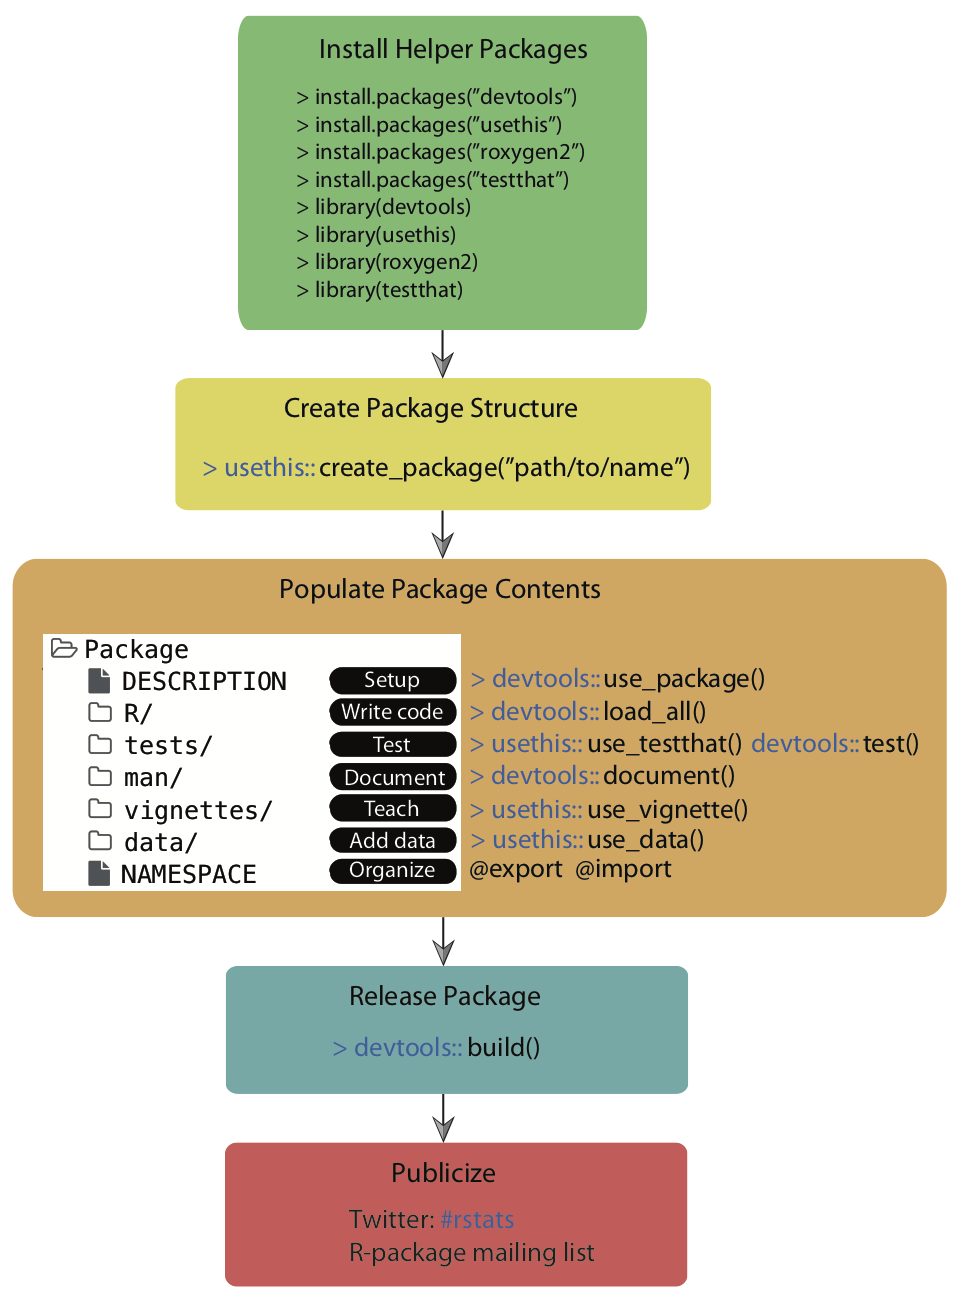
\includegraphics{images/package_workflow2.png}
\caption{}
\end{figure}

As a quick reminder, you can find the \texttt{devex} example package
linked \href{https://github.com/IQSS/Rbuild/tree/master/devex}{here, on
GitHub}, if you'd like to look through it while reading the guide.

\section{File Paths}\label{file-paths}

The paths used to locate files differ between UNIX (e.g., MacOS, Linux)
and Windows based operating systems. Windows systems used a single
backslash \texttt{\textbackslash{}}, while UNIX systems use a single
forward slash \texttt{/} to delimit files or directories in the path. R
follows the UNIX convention of using forward slashes, but forces this on
Window's users too. So, file paths should look like this:

\begin{enumerate}
\def\labelenumi{\arabic{enumi}.}
\tightlist
\item
  MacOS and Linux
\end{enumerate}

\texttt{\textasciitilde{}/Documents/myproject/myRfile.R}

\begin{enumerate}
\def\labelenumi{\arabic{enumi}.}
\setcounter{enumi}{1}
\tightlist
\item
  Windows
\end{enumerate}

\texttt{C:/Documents/myproject/myRfile.R}

In the examples provided in this guide, we will show MacOS file paths.
If you're using Windows, you will need to modify these paths slightly to
show the drive letter at the beginning, followed by a colon.

\section{Downloading Development
Tools}\label{downloading-development-tools}

Before we get started, you'll want to download four packages that are
extremely useful for package development. For Mac/Linux users, head to
the R Gui (or your favorite IDE) and run the code below to download the
packages. If you are prompted to choose a CRAN mirror for your session,
simply pick the mirror closest to your location.

\begin{Shaded}
\begin{Highlighting}[]
\KeywordTok{install.packages}\NormalTok{(}\StringTok{'devtools'}\NormalTok{)}
\KeywordTok{install.packages}\NormalTok{(}\StringTok{'usethis'}\NormalTok{)}
\KeywordTok{install.packages}\NormalTok{(}\StringTok{'roxygen2'}\NormalTok{)}
\KeywordTok{install.packages}\NormalTok{(}\StringTok{'testthat'}\NormalTok{)}
\end{Highlighting}
\end{Shaded}

If you are using Windows, prior to running the above code, you will need
to install ``RTools'' by following these instructions:

\begin{enumerate}
\def\labelenumi{\arabic{enumi}.}
\item
  Go to \url{https://cran.rstudio.com/} and select ``Download R for
  Windows.''
\item
  Click ``RTools'' and download the latest version of the tools (or the
  tools that are compatible with your version of R).
\item
  Let the installer run itself (the defaults are fine).
\end{enumerate}

\section{Initializing the Package}\label{initializing-the-package}

Now we can begin to walk through the process of creating an R package.
The first thing you'll always want to do is run the following function
to initialize the package:

\begin{Shaded}
\begin{Highlighting}[]
\NormalTok{usethis}\OperatorTok{::}\KeywordTok{create_package}\NormalTok{(}\StringTok{'path/to/desired/location/packagename'}\NormalTok{)}
\end{Highlighting}
\end{Shaded}

Note that the path specified by \texttt{usethis::create\_package()} must
currently be empty, otherwise \texttt{usethis} will throw an error.
Successfully running this function will create a couple of important
files which constitute a skeletal outline of the package. In particular,
it will create:

\begin{enumerate}
\def\labelenumi{\arabic{enumi}.}
\tightlist
\item
  An `R' subdirectory in the root of your specified directory, which is
  where all of core the R code of your package will live.
\item
  A DESCRIPTION file, which will come with a couple of preset fields.
\item
  A NAMESPACE file.
\end{enumerate}

You can then set the working directory for your project to an ``active''
status:

\begin{Shaded}
\begin{Highlighting}[]
\NormalTok{usethis}\OperatorTok{::}\KeywordTok{proj_set}\NormalTok{(}\StringTok{'path/to/desired/location/packagename'}\NormalTok{)}
\end{Highlighting}
\end{Shaded}

Once you've set up the basic structure of your package, you can start
modifying files and writing it in earnest!

\section{The DESCRIPTION}\label{the-description}

The DESCRIPTION file gives an extremely brief overview to the package.
It includes critical information such as the author of the package, the
title, a very short summary of its purpose, and the licensing
information. Open the ``DESCRIPTION'' file using your favorite text
editor in order to inspect and edit its contents.

DESCRIPTION is a DCF file (Debian control format). This file format may
be unfamiliar, but it's quite simple. Each line contains a field name
and value, separated by a colon. Sometimes, values are long enough to
require multiple lines, in which case they are indented by four spaces.
For example, the DESCRIPTION file for a newly created package will look
like this:

\begin{figure}
\centering
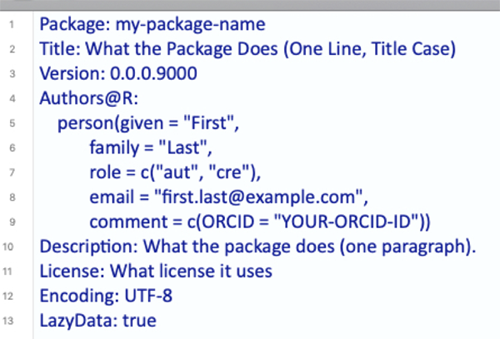
\includegraphics{images/packageSS/description_blank.png}
\caption{}
\end{figure}

Let's go through the fields and discuss what they mean. The first seven
fields listed are mandatory, meaning that if you do not include them,
the development environment will throw an error later on when you're
trying to build your package.

\begin{enumerate}
\def\labelenumi{\arabic{enumi}.}
\tightlist
\item
  \textbf{Package}: This is the name of the package. It should match the
  package name you chose earlier, and you should probably just leave
  this as is.
\item
  \textbf{Title}: A short but more descriptive title of your package
  than its name.
\item
  \textbf{Version}: The version of your package. Since you're creating
  this package for the first time, presumably it's version 0.1.0.
\item
  \textbf{Authors}: Here, you should add in your given and family names,
  role, email, and (optionally) your ORCID.
\item
  \textbf{Description}: This should be a one-paragraph
  \emph{comprehensive} description of the package. It is necessarily a
  high level-description, but it should be a complete one.
\item
  \textbf{License}: You should add in a License, which describes how
  others can legally use the package. Most of the time (especially in
  the US), you should write `CC0' in the License field, which implies
  that the package is open for all use, and you have relinquished all
  your rights to it. For more information on various licensing options,
  click
  \href{https://cran.r-project.org/doc/manuals/r-release/R-exts.html\#Licensing}{this
  link}.
\item
  \textbf{Encoding}: Just leave this as ``UTF-8''; discussing what
  encodings are isn't super important for this guide. If you're dying to
  learn about encodings, visit
  \href{https://www.w3.org/International/questions/qa-what-is-encoding}{this
  webpage}.
\item
  \textbf{LazyData}: Just leave this as `true', which ensures that if
  you include any data with your package (which you frequently will),
  when another user loads your package, they won't automatically load up
  the data, but will only load it if it becomes necessary during their
  use. This option reduces the amount of RAM users have to expend when
  loading packages, especially if you are planning to include a lot of
  data with your package.
\end{enumerate}

(Note all of the fields from this point on are optional, but
encouraged!)

\begin{enumerate}
\def\labelenumi{\arabic{enumi}.}
\setcounter{enumi}{8}
\tightlist
\item
  \textbf{Type}: This describes what type of project you're creating -
  in this case, because you're creating a package, you should write
  ``Package.''
\item
  \textbf{Date}: The date, in YYYY-MM-DD fashion.
\item
  \textbf{RoxygenNote}: Roxygen will automatically fill in the version
  of \texttt{Roxygen2} used to build the package in this field.
\end{enumerate}

(These fields are exceptionally important if you are building a package
using tools from other packages)

\begin{enumerate}
\def\labelenumi{\arabic{enumi}.}
\setcounter{enumi}{11}
\tightlist
\item
  \textbf{Imports}: In this field, you should list the packages which
  your package needs to function. Each package should be indented by two
  spaces, separated by a comma, and given its own line. For example, a
  pacakge which requires \texttt{ggplot2}, \texttt{nlme}, and
  \texttt{rpart} might have an `imports' field which looks like this:
\end{enumerate}

\begin{figure}
\centering
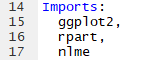
\includegraphics{images/packageSS/imports.PNG}
\caption{}
\end{figure}

\begin{enumerate}
\def\labelenumi{\arabic{enumi}.}
\setcounter{enumi}{12}
\tightlist
\item
  \textbf{Suggests}: Sometimes, your package will not really
  \emph{require} the use of other packages, but it might offer a couple
  of extra wrappers/functions with those other packages. When those
  extra functions aren't strictly necessary, it's a good idea to have
  your package \emph{suggest} imports. For example, a package which
  includes the following function should include \texttt{ggplot2} in the
  `suggests' part of the description.
\end{enumerate}

\begin{Shaded}
\begin{Highlighting}[]
\NormalTok{scalep <-}\StringTok{ }\ControlFlowTok{function}\NormalTok{(d, }\DataTypeTok{x=}\DecValTok{1}\NormalTok{)\{}
\NormalTok{  ...}
  \CommentTok{# If ggplot2 is available, use its qplot function - else, use the default hist function}
  \ControlFlowTok{if}\NormalTok{ (}\KeywordTok{requireNamespace}\NormalTok{(}\StringTok{"ggplot2"}\NormalTok{, }\DataTypeTok{quietly =} \OtherTok{TRUE}\NormalTok{)) \{}
\NormalTok{    ggplot2}\OperatorTok{::}\KeywordTok{qplot}\NormalTok{(r, }\DataTypeTok{geom=}\StringTok{'histogram'}\NormalTok{)}
\NormalTok{  \} }\ControlFlowTok{else}\NormalTok{ \{}
    \KeywordTok{hist}\NormalTok{(r)}
\NormalTok{  \}}
\NormalTok{  ...}
\NormalTok{\}}
\end{Highlighting}
\end{Shaded}

Here, the function \texttt{requireNameSpace()} checks if
\texttt{ggplot2} is available, and if not, the function uses the
(slightly less pretty) default histogram function.

Once you know which packages to list in the `suggests' section, you can
list them exactly the same way you'd list functions in the `imports'
section: each package is indented by two spaces, separated by a comma,
and gets its own line.

In general, it's best to suggest functions instead of requiring them if
you barely use them in your package. This will give users a bit more
flexibility, because it won't force them to download packages they will
probably never use.

\section{Writing Code}\label{writing-code}

\subsection{General Coding Guidelines}\label{general-coding-guidelines}

All of your code should be in scripts in the `R' file created in the
package development environment, as shown below:

\begin{figure}
\centering
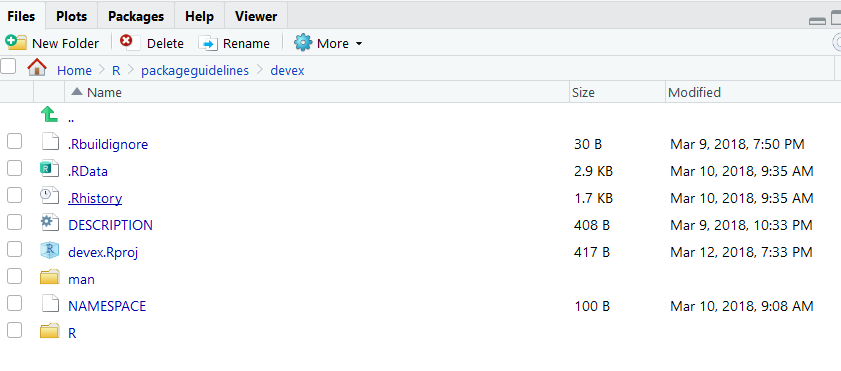
\includegraphics{images/packageSS/code1.PNG}
\caption{}
\end{figure}

The coding you will do in package development is slightly different than
the coding you'll normally do when writing R scripts. This is for a
couple of reasons:

\begin{enumerate}
\def\labelenumi{\arabic{enumi}.}
\tightlist
\item
  When you write a script and load that script using
  \texttt{source("script\_name")}, the code in the script runs when you
  load it (specifically, when you run the \texttt{source()} command). On
  the other hand, the code in a package is run when the package is
  \emph{built} on your computer. As a result, your code should mostly be
  focused on building functions, as opposed to a series of actions which
  the computer ought to take.
\item
  Unlike your personal scripts, other people will be using your package,
  and if your package is good, they'll be using it in ways you didn't
  anticipate. This means you ought to really try to make sure your code
  is as general as possible and can support a variety of approaches and
  implementations.
\item
  Also, because other people will be using your package, you should
  avoid modifying the global environment with your package. This means
  avoiding using functions like \texttt{require()}, \texttt{library()},
  or \texttt{source()}; instead, there are other alternatives which can
  accomplish the same goal without changing the global environment and
  potentially giving other users an unwanted surprise. For example,
  instead of using \texttt{library()} and \texttt{require()}, you should
  be listing your necessary imports in the DESCRIPTION file, as outlined
  above, and then R will make sure anyone who installs and loads your
  package also has any other packages your package depends on. The one
  catch is that you'll now have to append \texttt{packagename::} in
  front of the imported functions you want to use, otherwise R won't
  recognize them. For example, to use the \texttt{qplot()} function from
  the \texttt{ggplot2} package, the code should look like:
\end{enumerate}

\begin{Shaded}
\begin{Highlighting}[]
\NormalTok{ ...}
\NormalTok{scalep <-}\StringTok{ }\ControlFlowTok{function}\NormalTok{(d, }\DataTypeTok{x=}\DecValTok{1}\NormalTok{)\{}
\NormalTok{ ...}
\NormalTok{  ggplot2}\OperatorTok{::}\KeywordTok{qplot}\NormalTok{(r, }\DataTypeTok{geom=}\StringTok{'histogram'}\NormalTok{)}
\NormalTok{ ...}
\NormalTok{\}}
\end{Highlighting}
\end{Shaded}

The last thing you should know is that if you want your package to plot
things, you will have to surround the \texttt{plot()} commands with a
\texttt{print()} statement, like this:

\begin{Shaded}
\begin{Highlighting}[]
\NormalTok{ ...}
\NormalTok{scalep <-}\StringTok{ }\ControlFlowTok{function}\NormalTok{(d, }\DataTypeTok{x=}\DecValTok{1}\NormalTok{)\{}
\NormalTok{ ...}
  \KeywordTok{print}\NormalTok{(ggplot2}\OperatorTok{::}\KeywordTok{qplot}\NormalTok{(r, }\DataTypeTok{geom=}\StringTok{'histogram'}\NormalTok{))}
\NormalTok{ ...}
\NormalTok{\}}
\end{Highlighting}
\end{Shaded}

You should also take care to organize your functions properly. It's
probably a bad idea to stick them all into one script and title it
``functions.'' Instead, you should organize functions by their purposes
- for example, a variety of loss functions might go into a single
script. Of course, some very complicated functions might deserve their
own script. The file names of the script should be descriptive - for
example, a script of loss functions might be named
``loss\_functions.R''.

\subsection{Code Style}\label{code-style}

Now let's talk about code style. These recommendations are shortened and
adapted from \href{http://r-pkgs.had.co.nz/r.html}{Hadley Wickham's
book}, which in turn were adapted from Google's style guide.

\begin{enumerate}
\def\labelenumi{\arabic{enumi}.}
\tightlist
\item
  \textbf{Comments}: Comments are the best way to make your code
  readable. In general, you should err on the side of commenting too
  much rather than too little, and your comments should explain the
  \emph{motivation} of your code as opposed to what your code actually
  does (although admittedly the line between those two things is a bit
  blurry). Moreover, you can use lines of `\#
  ---------------------------' or `\# ==================' to separate
  sections of your code. Here are some examples:
\end{enumerate}

\begin{Shaded}
\begin{Highlighting}[]
\CommentTok{# Returns the squared element-wise difference between two vectors}
\NormalTok{loss <-}\StringTok{ }\ControlFlowTok{function}\NormalTok{(x,y) \{}
\NormalTok{  error <-}\StringTok{ }\NormalTok{(x}\OperatorTok{-}\NormalTok{y)}\OperatorTok{**}\DecValTok{2}
  \KeywordTok{return}\NormalTok{(error)}
\NormalTok{\}}
\CommentTok{#---------------------------------------------------------------------------}

\CommentTok{# Takes the square root of any real number, returning a complex number}
\NormalTok{general_sqrt <-}\StringTok{ }\ControlFlowTok{function}\NormalTok{ (x) \{}
  \CommentTok{# Return the normal square root if x > 0}
  \ControlFlowTok{if}\NormalTok{ (x }\OperatorTok{>}\StringTok{ }\DecValTok{0} \OperatorTok{||}\StringTok{ }\NormalTok{x }\OperatorTok{==}\StringTok{ }\DecValTok{0}\NormalTok{) \{}
    \KeywordTok{return}\NormalTok{(}\KeywordTok{complex}\NormalTok{(}\DataTypeTok{real=}\KeywordTok{sqrt}\NormalTok{(x), }\DataTypeTok{imaginary=}\DecValTok{0}\NormalTok{))}
\NormalTok{  \}}
  \CommentTok{# Else return the complex square root}
  \ControlFlowTok{else}\NormalTok{ \{}
    \KeywordTok{return}\NormalTok{(}\KeywordTok{complex}\NormalTok{(}\DataTypeTok{real =} \DecValTok{0}\NormalTok{, }\DataTypeTok{imaginary =} \KeywordTok{sqrt}\NormalTok{(}\OperatorTok{-}\NormalTok{x)))}
\NormalTok{  \}}
\NormalTok{\}}
\end{Highlighting}
\end{Shaded}

\begin{enumerate}
\def\labelenumi{\arabic{enumi}.}
\setcounter{enumi}{1}
\tightlist
\item
  \textbf{Names}: Variable and function names should be descriptive but
  concise, and variable names should generally be nouns whereas function
  names tend to be verbs. Most R developers keep their function/variable
  names all lowercase and separate multiple words with underscores.
  There are no strict rules on this, but it's nice to be consistent with
  \emph{some} rules because it makes your code readable.
\end{enumerate}

\begin{Shaded}
\begin{Highlighting}[]
\CommentTok{# Bad example - function name}
\NormalTok{f <-}\StringTok{ }\ControlFlowTok{function}\NormalTok{(x) \{}
  \KeywordTok{return}\NormalTok{(}\KeywordTok{sqrt}\NormalTok{(x))}
\NormalTok{\}}

\CommentTok{# Good example - function name}
\NormalTok{take_sqrt <-}\StringTok{ }\ControlFlowTok{function}\NormalTok{(x)\{}
  \KeywordTok{return}\NormalTok{(}\KeywordTok{sqrt}\NormalTok{(x))}
\NormalTok{\}}

\CommentTok{# Bad example - variable name}
\NormalTok{s <-}\StringTok{ }\KeywordTok{read.table}\NormalTok{(path)}

\CommentTok{# Good example - variable name}
\NormalTok{car_data <-}\StringTok{ }\KeywordTok{read.table}\NormalTok{(path)}
\end{Highlighting}
\end{Shaded}

\begin{enumerate}
\def\labelenumi{\arabic{enumi}.}
\setcounter{enumi}{2}
\tightlist
\item
  \textbf{Curly Braces}: You should start a new line after you write an
  opening curly brace, and ending curly braces should get their own
  lines, unless you have an else clause or the line is exceptionally
  simple.
\end{enumerate}

\begin{Shaded}
\begin{Highlighting}[]
\CommentTok{# Bad examples}

\ControlFlowTok{if}\NormalTok{ (condition) \{}
  \KeywordTok{complicated_function}\NormalTok{(x)\} }\CommentTok{# Ending curly brace should get a new line}

\CommentTok{# Good examples}
\ControlFlowTok{if}\NormalTok{ (condition) \{}\KeywordTok{do}\NormalTok{(x)\} }\ControlFlowTok{else}\NormalTok{ \{}\KeywordTok{do}\NormalTok{(y)\}}

\ControlFlowTok{if}\NormalTok{ (condition) \{}
  \KeywordTok{complicated_function_call}\NormalTok{(arg1, arg2, arg3)}
\NormalTok{\} }\ControlFlowTok{else}\NormalTok{ \{}
  \KeywordTok{other_complex_function_call}\NormalTok{(arg7, arg3, arg5)}
\NormalTok{\}}
\end{Highlighting}
\end{Shaded}

As always, you can break the rules if you have a good reason to.

Different organizations and programmers may have different styles, but
in general, you should remember:

\begin{enumerate}
\def\labelenumi{\arabic{enumi}.}
\tightlist
\item
  Your goal should always be to make your code readable!
\item
  Whatever style guide you follow, follow it \emph{consistently}.
\item
  When in doubt, follow the conventions of the organization you're
  working for.
\end{enumerate}

\subsection{Warnings and Simplicity}\label{warnings-and-simplicity}

Consider the case of the \texttt{scalep()} function, which currently
takes a 2-column dataframe as an input, divides the second column by the
first, and returns/graphs some scaled proportion of the quotient vector.
One version of this function, which follows almost all of the guidelines
above, might look like this:

\begin{Shaded}
\begin{Highlighting}[]
\NormalTok{scalep <-}\StringTok{ }\ControlFlowTok{function}\NormalTok{(d, }\DataTypeTok{x=}\DecValTok{1}\NormalTok{)\{}

  \CommentTok{# Intialize resulting vector}
\NormalTok{  result <-}\StringTok{ }\KeywordTok{c}\NormalTok{()}

  \CommentTok{# Iterate through and divide column 2 of d by column 1 of d}
\NormalTok{  i <-}\StringTok{ }\DecValTok{0}
  \ControlFlowTok{while}\NormalTok{(i }\OperatorTok{<}\StringTok{ }\KeywordTok{length}\NormalTok{(d[ ,}\DecValTok{1}\NormalTok{]) }\OperatorTok{+}\StringTok{ }\DecValTok{1}\NormalTok{)\{}
\NormalTok{    row <-}\StringTok{ }\NormalTok{d[i,]}
\NormalTok{    result <-}\StringTok{ }\KeywordTok{append}\NormalTok{(result, row[[}\DecValTok{2}\NormalTok{]]}\OperatorTok{/}\NormalTok{row[[}\DecValTok{1}\NormalTok{]])}
\NormalTok{    i <-}\StringTok{ }\NormalTok{i }\OperatorTok{+}\StringTok{ }\DecValTok{1}
\NormalTok{  \}}

  \CommentTok{# Print the graph using either ggplot2 or the hist function}
  \ControlFlowTok{if}\NormalTok{ (}\KeywordTok{requireNamespace}\NormalTok{(}\StringTok{"ggplot2"}\NormalTok{, }\DataTypeTok{quietly =} \OtherTok{TRUE}\NormalTok{)) \{}
    \KeywordTok{print}\NormalTok{(ggplot2}\OperatorTok{::}\KeywordTok{qplot}\NormalTok{(result, }\DataTypeTok{geom=}\StringTok{'histogram'}\NormalTok{))}
\NormalTok{  \} }\ControlFlowTok{else}\NormalTok{ \{}
    \KeywordTok{print}\NormalTok{(}\KeywordTok{hist}\NormalTok{(result))}
\NormalTok{  \}}

  \CommentTok{# Return the result, multiplying by the optional scalar}
\NormalTok{  result <-}\StringTok{ }\NormalTok{x}\OperatorTok{*}\NormalTok{result}
  \KeywordTok{return}\NormalTok{(result)}
\NormalTok{\}}
\end{Highlighting}
\end{Shaded}

However, this function still has a couple of problems. It's not super
easy to use because (a) it's understandably hard for other programmers
to remember which column is divided by which and (b) there's a simpler
way to accomplish the code above which will make it more readable.
Specifically, it might be easier to just have arguments called `factors'
and `divisors' and then divide them, like this:

\begin{Shaded}
\begin{Highlighting}[]
\NormalTok{scalep <-}\StringTok{ }\ControlFlowTok{function}\NormalTok{(factors, divisors, }\DataTypeTok{constant =} \DecValTok{1}\NormalTok{) \{}

  \CommentTok{# Divide and multiply by optional scalar}
\NormalTok{  proportions <-}\StringTok{ }\NormalTok{constant}\OperatorTok{*}\NormalTok{factors}\OperatorTok{/}\NormalTok{divisors}

  \CommentTok{# Print the graph using either ggplot2 or the hist function}
  \ControlFlowTok{if}\NormalTok{ (}\KeywordTok{requireNamespace}\NormalTok{(}\StringTok{"ggplot2"}\NormalTok{, }\DataTypeTok{quietly =} \OtherTok{TRUE}\NormalTok{)) \{}
    \KeywordTok{print}\NormalTok{(ggplot2}\OperatorTok{::}\KeywordTok{qplot}\NormalTok{(proportions, }\DataTypeTok{geom=}\StringTok{'histogram'}\NormalTok{))}
\NormalTok{  \} }\ControlFlowTok{else}\NormalTok{ \{}
    \KeywordTok{print}\NormalTok{(}\KeywordTok{hist}\NormalTok{(proportions))}
\NormalTok{  \}}

  \CommentTok{# Return the result}
  \KeywordTok{return}\NormalTok{(proportions)}
\NormalTok{\}}
\end{Highlighting}
\end{Shaded}

The new argument structure will make it a bit easier to use. Similarly,
the new structure simplifies the code, making it a bit more readable.
However, it does pose one problem: whereas the previous structure
mandated that the two vectors be the same length (because they were part
of a dataframe), in this function, the two vectors might not be the same
length and the function would not always throw an error (specifically,
if `factors' has a length which is is an integer multiple of the length
of `divisors', R will not warn the user at all). This problem is a type
of \textbf{silent error} (silent errors are bugs which do not issue
warnings or errors). Silent errors are terrible because they make
bug-hunting extremely difficult: in large repositories of code, it
becomes nearly impossible to find which specific line is causing
problems without some kind of warning. Thus, it's also worth adding in a
couple of lines to warn the user if the factors and divisors are of
different lengths, as is outlined below:

\begin{Shaded}
\begin{Highlighting}[]
  \CommentTok{# Check divisors and factors are the same length}
  \ControlFlowTok{if}\NormalTok{ (}\KeywordTok{length}\NormalTok{(divisors) }\OperatorTok{!=}\StringTok{ }\KeywordTok{length}\NormalTok{(factors)) \{}
    \KeywordTok{warning}\NormalTok{(}\StringTok{'Length of divisors argument is not equal to length of factors argument'}\NormalTok{)}
\NormalTok{  \}}
\end{Highlighting}
\end{Shaded}

Lastly, it's just worth adding an extra optional argument to let your
users turn off the graphing feature of \texttt{scalep()}, just to make
the function more useable, as follows:

\begin{Shaded}
\begin{Highlighting}[]
\NormalTok{scalep <-}\StringTok{ }\ControlFlowTok{function}\NormalTok{(factors, divisors, }\DataTypeTok{constant =} \DecValTok{1}\NormalTok{, }\DataTypeTok{graph =} \OtherTok{FALSE}\NormalTok{) \{}

\NormalTok{  ...}

  \CommentTok{# If graph = True, print the graph using either ggplot2 or the hist function}
  \ControlFlowTok{if}\NormalTok{ (}\KeywordTok{requireNamespace}\NormalTok{(}\StringTok{"ggplot2"}\NormalTok{, }\DataTypeTok{quietly =} \OtherTok{TRUE}\NormalTok{) }\OperatorTok{&}\StringTok{ }\NormalTok{graph) \{}
    \KeywordTok{print}\NormalTok{(ggplot2}\OperatorTok{::}\KeywordTok{qplot}\NormalTok{(proportions, }\DataTypeTok{geom=}\StringTok{'histogram'}\NormalTok{))}
\NormalTok{  \} }\ControlFlowTok{else} \ControlFlowTok{if}\NormalTok{ (graph) \{}
    \KeywordTok{print}\NormalTok{(}\KeywordTok{hist}\NormalTok{(proportions))}
\NormalTok{  \}}

\NormalTok{  ...}
\end{Highlighting}
\end{Shaded}

To summarize, this subsection thus contained three core ideas: (1) make
your code simple, (2) make it easy to use by labeling arguments, and (3)
always avoid silent errors.

\subsection{Loading Your Code}\label{loading-your-code}

If you've finished writing your code and want to play with it a little
bit, you can use the following function:

\begin{Shaded}
\begin{Highlighting}[]
\NormalTok{devtools}\OperatorTok{::}\KeywordTok{load_all}\NormalTok{()}
\end{Highlighting}
\end{Shaded}

which (according to its documentation) ``roughly simulates what happens
when a package is installed and loaded with library.'' As we'll see in
the \protect\hyperlink{releasing-your-package}{build},
\protect\hyperlink{testing}{testing}, and
\href{./integrated-development-environments.html\#ex-building-packages}{RStudio}
sections, there are better ways to simulate the user experience and test
your code, but \texttt{load\_all()} is often a useful intermediate step.

\hypertarget{testing}{\section{Testing}\label{testing}}

\subsection{Why should you test?}\label{why-should-you-test}

Suppose an imaginary programmer named Grace has created a package and
has been using it for a while, but she decides she'd like to modify one
function to improve it. She modifies her function, tests it a bit, and
then publishes a new version of the package. Yet two weeks later,
another imaginary programmer named Carlos discovers that the changes she
made created a bug in \emph{another} function in the package! This
situation is very annoying, especially if Carlos has no idea what has
caused the bug or how to fix it. Unfortunately, it's also an extremely
common problem.

The solution to problems like this is to test your package
\emph{systematically} and \emph{automatically}. If Grace had rigorously
tested the entire package before publishing it, Carlos would never have
had to deal with the new bug- Grace would have found out immediately. In
other words, a good principle in package development is to make sure
your code \emph{fails as fast as possible,} so you can find out and fix
it. Of course, all programmers test their code, but not everyone tests
systematically and automatically.

\subsection{What are unit tests?}\label{what-are-unit-tests}

Tests compare the \emph{expected} output of a block of code to its
\emph{actual} output. For example, the following test tests whether the
``generalized square root'' function actually returns \(2\) as the
square root of \(4\).

\begin{Shaded}
\begin{Highlighting}[]
\KeywordTok{expect_equal}\NormalTok{(}\KeywordTok{general_sqrt}\NormalTok{(}\DecValTok{4}\NormalTok{), }\KeywordTok{complex}\NormalTok{(}\DataTypeTok{real =} \DecValTok{2}\NormalTok{, }\DataTypeTok{imaginary =} \DecValTok{0}\NormalTok{))}
\end{Highlighting}
\end{Shaded}

\emph{Unit tests} usually run on the computer of the developer who is
modifying a package and also should run automatically upon building a
package.

We'll talk a little more about how exactly to create tests below, but
hopefully this makes the general concept clear (you've also probably
been using the general concept as you program).

\subsection{Setting up the testing
environment}\label{setting-up-the-testing-environment}

Creating unit tests is actually quite easy, thanks to a package called
\texttt{testthat} which works in combination with \texttt{usethis}. To
begin, you should run the following command in your favorite IDE, or
even in the R Gui:

\begin{Shaded}
\begin{Highlighting}[]
\NormalTok{usethis}\OperatorTok{::}\KeywordTok{use_testthat}\NormalTok{()}
\end{Highlighting}
\end{Shaded}

This will do a couple of things. First, it will add \texttt{testthat} to
the Suggests part of the DESCRIPTION, which will help other
collaborators know to use \texttt{testthat} when modifying/working on
the package. It will also create a `tests/testthat' directory in your
project, as well a file called `test/testthat.R', as shown below.

\begin{figure}
\centering
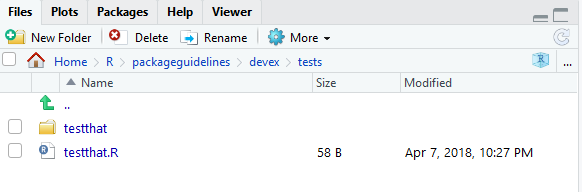
\includegraphics{images/testSS/devtoolstestthat.PNG}
\caption{}
\end{figure}

\subsection{Expectations}\label{expectations}

Before discussing how to write unit tests, we need to properly describe
an expectation. An expectation tests whether the actual output of a
single function call is what the developer expected. The
\texttt{testthat} package has a number of functions which compare
outputs to expected values. When calling one of these functions, one of
two things can happen:

\begin{enumerate}
\def\labelenumi{\arabic{enumi}.}
\tightlist
\item
  If the actual output matches the expectation, nothing will happen!
\item
  If the actual output does not match the expectation, it will throw an
  error.
\end{enumerate}

For example, \texttt{expect\_equal()} uses the base R function
\texttt{all.equal()} to check whether an output is (approximately) equal
to an expectation. In the following code, the first function call will
do nothing - the second function call will throw an error, displayed
below.

\begin{Shaded}
\begin{Highlighting}[]
\KeywordTok{library}\NormalTok{(testthat)}
\NormalTok{testthat}\OperatorTok{::}\KeywordTok{expect_equal}\NormalTok{(}\DecValTok{2}\NormalTok{, }\DecValTok{2}\NormalTok{)}
\NormalTok{testthat}\OperatorTok{::}\KeywordTok{expect_equal}\NormalTok{(}\DecValTok{2}\NormalTok{, }\DecValTok{4}\NormalTok{)}
\end{Highlighting}
\end{Shaded}

\begin{figure}
\centering

\includegraphics{images/testSS/expectationerror.PNG}
\caption{}
\end{figure}

Here's an (abbreviated) list of the expectation functions:

\begin{enumerate}
\def\labelenumi{\arabic{enumi}.}
\tightlist
\item
  \textbf{expect\_equal}, as aforementioned, checks equality using the
  ``all.equal()'' base function.
\item
  \textbf{expect\_identical} checks equality using the
  \texttt{identical()} base function. Generally, it's better to use
  \texttt{expect\_equal()} because lots of R functions use numerical
  approximations which will cause expect\_identical to fail when you
  don't want it to.
\item
  \textbf{expect\_match}, \textbf{expect\_output},
  \textbf{expect\_message}, \textbf{expect\_warning}, and
  \textbf{expect\_error} all respectively test whether a string, output,
  warning, or error match a regular expression. For example, the
  following two expectations functions will not throw errors:
\end{enumerate}

\begin{Shaded}
\begin{Highlighting}[]
\NormalTok{testthat}\OperatorTok{::}\KeywordTok{expect_match}\NormalTok{(}\StringTok{'hello1234'}\NormalTok{, }\StringTok{'hello'}\NormalTok{)}
\NormalTok{testthat}\OperatorTok{::}\KeywordTok{expect_warning}\NormalTok{(}\KeywordTok{sqrt}\NormalTok{(}\OperatorTok{-}\DecValTok{2}\NormalTok{), }\StringTok{'NaNs produced'}\NormalTok{)}
\end{Highlighting}
\end{Shaded}

The tests do not fail because (i) `hello1234' contains `hello' and (ii)
the error message produced by \texttt{sqrt(-2)} contains the phrase
`NaNs produced'.

\begin{enumerate}
\def\labelenumi{\arabic{enumi}.}
\setcounter{enumi}{3}
\tightlist
\item
  \textbf{expect\_is} tests whether an object inherits from a class,
  specified in quotes. For example, the following test passes:
\end{enumerate}

\begin{Shaded}
\begin{Highlighting}[]
\NormalTok{testthat}\OperatorTok{::}\KeywordTok{expect_is}\NormalTok{(}\KeywordTok{sqrt}\NormalTok{(}\DecValTok{2}\NormalTok{), }\StringTok{'numeric'}\NormalTok{)}
\end{Highlighting}
\end{Shaded}

\begin{enumerate}
\def\labelenumi{\arabic{enumi}.}
\setcounter{enumi}{4}
\tightlist
\item
  \textbf{expect\_true} and \textbf{expect\_false} respectively expect a
  statement to evaluate to TRUE or FALSE.
\end{enumerate}

\subsection{Structure and Location of Unit
Tests}\label{structure-and-location-of-unit-tests}

Each \emph{unit test} (which is written in an R script) should use a
couple of expectations to test a single core function. It should use the
function \texttt{test\_that()} (from the \texttt{testthat} package).
\texttt{test\_that()} takes two parameters: a string, which describes
the test, and a couple of expectations, surrounded by curly braces. For
example, the following code will test whether the
\texttt{general\_sqrt()} function from the \texttt{devex} package
returns a complex number.

\begin{Shaded}
\begin{Highlighting}[]
\KeywordTok{test_that}\NormalTok{(}\StringTok{"Returns complex number"}\NormalTok{, \{}
  \KeywordTok{expect_is}\NormalTok{(}\KeywordTok{general_sqrt}\NormalTok{(}\OperatorTok{-}\DecValTok{2}\NormalTok{), }\StringTok{'complex'}\NormalTok{)}
  \KeywordTok{expect_is}\NormalTok{(}\KeywordTok{general_sqrt}\NormalTok{(}\DecValTok{2}\NormalTok{), }\StringTok{'complex'}\NormalTok{)}
  \KeywordTok{expect_is}\NormalTok{(}\KeywordTok{general_sqrt}\NormalTok{(}\DecValTok{0}\NormalTok{), }\StringTok{'complex'}\NormalTok{)}
\NormalTok{\})}
\end{Highlighting}
\end{Shaded}

Multiple tests with similar functions should be put in the same file,
and those test files must be put in the tests/testthat/ directory.
Moreover, their name must start with the word `test' - this will help R
automatically run your tests for you. For example, in the \texttt{devex}
package, there are two very simple helper functions
(\texttt{general\_sqrt()} and \texttt{loss()}) and one moderately
complex function (\texttt{scalep()}). As a result, the \texttt{devex}
package has exactly two testing files: one called `testhelpers', which
tests the helper functions, and another called `testscalep', which tests
the \texttt{scalep()} function. The `testhelpers' file looks like this:

\begin{Shaded}
\begin{Highlighting}[]
\KeywordTok{library}\NormalTok{(devex)}
\KeywordTok{context}\NormalTok{(}\StringTok{"generalized sqrt and loss"}\NormalTok{)}

\CommentTok{# Generalized sqrt ---------------------------------------}

\KeywordTok{test_that}\NormalTok{(}\StringTok{"Returns complex number"}\NormalTok{, \{}
  \KeywordTok{expect_is}\NormalTok{(}\KeywordTok{general_sqrt}\NormalTok{(}\OperatorTok{-}\DecValTok{2}\NormalTok{), }\StringTok{'complex'}\NormalTok{)}
  \KeywordTok{expect_is}\NormalTok{(}\KeywordTok{general_sqrt}\NormalTok{(}\DecValTok{2}\NormalTok{), }\StringTok{'complex'}\NormalTok{)}
  \KeywordTok{expect_is}\NormalTok{(}\KeywordTok{general_sqrt}\NormalTok{(}\DecValTok{0}\NormalTok{), }\StringTok{'complex'}\NormalTok{)}
\NormalTok{\})}

\KeywordTok{test_that}\NormalTok{(}\StringTok{"Returns correct sqrt"}\NormalTok{, \{}
  \KeywordTok{expect_equal}\NormalTok{(}\KeywordTok{general_sqrt}\NormalTok{(}\OperatorTok{-}\FloatTok{1.53}\NormalTok{), }\KeywordTok{complex}\NormalTok{(}\DataTypeTok{real =} \DecValTok{0}\NormalTok{, }\DataTypeTok{imaginary =} \KeywordTok{sqrt}\NormalTok{(}\FloatTok{1.53}\NormalTok{)))}
  \KeywordTok{expect_equal}\NormalTok{(}\KeywordTok{general_sqrt}\NormalTok{(}\OperatorTok{-}\DecValTok{2}\NormalTok{), }\KeywordTok{complex}\NormalTok{(}\DataTypeTok{real =} \DecValTok{0}\NormalTok{, }\DataTypeTok{imaginary =} \KeywordTok{sqrt}\NormalTok{(}\DecValTok{2}\NormalTok{)))}
\NormalTok{\})}

\KeywordTok{test_that}\NormalTok{(}\StringTok{"Warnings for vectors of length > 1"}\NormalTok{, \{}
  \KeywordTok{expect_warning}\NormalTok{(}\KeywordTok{general_sqrt}\NormalTok{(}\KeywordTok{c}\NormalTok{(}\DecValTok{2}\NormalTok{, }\DecValTok{0}\NormalTok{)))}
  \KeywordTok{expect_warning}\NormalTok{(}\KeywordTok{general_sqrt}\NormalTok{(}\KeywordTok{c}\NormalTok{(}\OperatorTok{-}\DecValTok{2}\NormalTok{, }\DecValTok{0}\NormalTok{, }\DecValTok{2}\NormalTok{)), }\StringTok{'NaNs produced'}\NormalTok{)}
\NormalTok{\})}

\CommentTok{# Loss ---------------------------------------------------}

\KeywordTok{test_that}\NormalTok{(}\StringTok{"Returns correct loss"}\NormalTok{, \{}
  \KeywordTok{expect_equal}\NormalTok{(}\KeywordTok{loss}\NormalTok{(}\DecValTok{0}\NormalTok{, }\DecValTok{3}\NormalTok{), }\DecValTok{9}\NormalTok{)}
  \KeywordTok{expect_equal}\NormalTok{(}\KeywordTok{loss}\NormalTok{(}\KeywordTok{c}\NormalTok{(}\DecValTok{1}\NormalTok{, }\DecValTok{1}\NormalTok{, }\DecValTok{1}\NormalTok{), }\KeywordTok{c}\NormalTok{(}\DecValTok{1}\NormalTok{, }\DecValTok{2}\NormalTok{, }\DecValTok{3}\NormalTok{)), }\KeywordTok{c}\NormalTok{(}\DecValTok{0}\NormalTok{, }\DecValTok{1}\NormalTok{, }\DecValTok{4}\NormalTok{))}
  \KeywordTok{expect_equal}\NormalTok{(}\KeywordTok{loss}\NormalTok{(}\KeywordTok{c}\NormalTok{(}\OperatorTok{-}\DecValTok{1}\NormalTok{, }\OperatorTok{-}\DecValTok{5}\NormalTok{, }\OperatorTok{-}\DecValTok{2}\NormalTok{), }\KeywordTok{c}\NormalTok{(}\DecValTok{0}\NormalTok{, }\DecValTok{0}\NormalTok{, }\DecValTok{0}\NormalTok{)), }\KeywordTok{c}\NormalTok{(}\DecValTok{1}\NormalTok{, }\DecValTok{25}\NormalTok{, }\DecValTok{4}\NormalTok{))}
\NormalTok{\})}
\end{Highlighting}
\end{Shaded}

Each test file, as demonstrated above, needs to load the package of
interest (using \texttt{library()} is fine) and also should supply a
string which succinctly describes the general purpose of all of the
tests in the test file to the \texttt{context()} function.

You can run all of the tests in the test/testthat directory by running
the following \texttt{devtools} function:

\begin{Shaded}
\begin{Highlighting}[]
\NormalTok{devtools}\OperatorTok{::}\KeywordTok{test}\NormalTok{()}
\end{Highlighting}
\end{Shaded}

If any test throws an error, R will report two things. First, it will
report the string given in the test which was given to the
\texttt{test\_that()} function call. Second, it will report the filename
of the test file as well as the line of code that threw an error. For
example, running the above tests yields the following result:

\begin{figure}
\centering
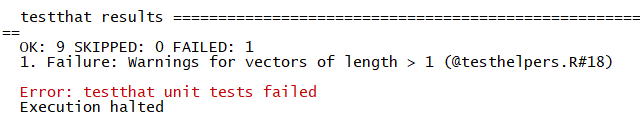
\includegraphics{images/testSS/testthaterror1.PNG}
\caption{}
\end{figure}

This indicates that line 18 of testhelpers.R failed in the test
``Warnings for vectors of length \textgreater{} 1.'' Looking at the test
code reveals that the \texttt{general\_sqrt()} function does not return
a warning for positive vectors of length greater than one.

\begin{Shaded}
\begin{Highlighting}[]
\KeywordTok{expect_warning}\NormalTok{(}\KeywordTok{general_sqrt}\NormalTok{(}\KeywordTok{c}\NormalTok{(}\DecValTok{2}\NormalTok{, }\DecValTok{0}\NormalTok{)))}
\end{Highlighting}
\end{Shaded}

To fix this, it might be worth adding in an extra line or two which
ensures that the input to \texttt{general\_sqrt()} is as it should be
(to prevent users from getting unexpected results).

\subsection{Writing Good Tests}\label{writing-good-tests}

Good tests have a couple of characteristics.

\textbf{First}, good tests have high \emph{coverage,} meaning that they
test a large percentage of the lines of code of the package. For
example, the code for the \texttt{general\_sqrt()} function is as
follows:

\begin{Shaded}
\begin{Highlighting}[]
\CommentTok{# This function takes the complex square root of real numbers}

\NormalTok{general_sqrt <-}\StringTok{ }\ControlFlowTok{function}\NormalTok{ (x)\{}

  \CommentTok{# Issue warning for longer vectors}
  \ControlFlowTok{if}\NormalTok{ (}\KeywordTok{length}\NormalTok{(x) }\OperatorTok{>}\StringTok{ }\DecValTok{1}\NormalTok{) \{}
    \KeywordTok{warning}\NormalTok{(}\StringTok{'Argument of general_sqrt has length greater than 1'}\NormalTok{)}
\NormalTok{  \}}

  \CommentTok{# Return the normal square root if x > 0}
  \ControlFlowTok{if}\NormalTok{ (x }\OperatorTok{>}\StringTok{ }\DecValTok{0} \OperatorTok{||}\StringTok{ }\NormalTok{x }\OperatorTok{==}\StringTok{ }\DecValTok{0}\NormalTok{)\{}
    \KeywordTok{return}\NormalTok{(}\KeywordTok{complex}\NormalTok{(}\DataTypeTok{real =} \KeywordTok{sqrt}\NormalTok{(x), }\DataTypeTok{imaginary =} \DecValTok{0}\NormalTok{))}
\NormalTok{  \}}

  \CommentTok{# Else return the complex square root}

  \ControlFlowTok{else}\NormalTok{ \{}
    \KeywordTok{return}\NormalTok{(}\KeywordTok{complex}\NormalTok{(}\DataTypeTok{real =} \DecValTok{0}\NormalTok{, }\DataTypeTok{imaginary =} \KeywordTok{sqrt}\NormalTok{(}\OperatorTok{-}\NormalTok{x)))}
\NormalTok{  \}}

\NormalTok{\}}
\end{Highlighting}
\end{Shaded}

The following test has low coverage for the \texttt{general\_sqrt()}
function:

\begin{Shaded}
\begin{Highlighting}[]
\KeywordTok{test_that}\NormalTok{(}\StringTok{"Returns correct sqrt"}\NormalTok{, \{}
  \KeywordTok{expect_equal}\NormalTok{(}\KeywordTok{general_sqrt}\NormalTok{(}\OperatorTok{-}\FloatTok{1.53}\NormalTok{), }\KeywordTok{complex}\NormalTok{(}\DataTypeTok{real =} \DecValTok{0}\NormalTok{, }\DataTypeTok{imaginary =} \KeywordTok{sqrt}\NormalTok{(}\FloatTok{1.53}\NormalTok{)))}
  \KeywordTok{expect_equal}\NormalTok{(}\KeywordTok{general_sqrt}\NormalTok{(}\OperatorTok{-}\DecValTok{2}\NormalTok{), }\KeywordTok{complex}\NormalTok{(}\DataTypeTok{real =} \DecValTok{0}\NormalTok{, }\DataTypeTok{imaginary =} \KeywordTok{sqrt}\NormalTok{(}\DecValTok{2}\NormalTok{)))}
\NormalTok{\})}
\end{Highlighting}
\end{Shaded}

because it only tests whether \texttt{general\_sqrt()} returns the
correct square root for negative numbers. This test thus only covers
half of the code in \texttt{general\_sqrt()}, because the mechanism for
dealing with nonnegative numbers is entirely separate. The following
test is a better example, because it tests both positive and negative
numbers.

\begin{Shaded}
\begin{Highlighting}[]
\KeywordTok{test_that}\NormalTok{(}\StringTok{"Returns correct sqrt"}\NormalTok{, \{}
  \KeywordTok{expect_equal}\NormalTok{(}\KeywordTok{general_sqrt}\NormalTok{(}\FloatTok{1.53}\NormalTok{), }\KeywordTok{complex}\NormalTok{(}\DataTypeTok{real =} \KeywordTok{sqrt}\NormalTok{(}\FloatTok{1.53}\NormalTok{), }\DataTypeTok{imaginary =} \DecValTok{0}\NormalTok{))}
  \KeywordTok{expect_equal}\NormalTok{(}\KeywordTok{general_sqrt}\NormalTok{(}\OperatorTok{-}\DecValTok{2}\NormalTok{), }\KeywordTok{complex}\NormalTok{(}\DataTypeTok{real =} \DecValTok{0}\NormalTok{, }\DataTypeTok{imaginary =} \KeywordTok{sqrt}\NormalTok{(}\DecValTok{2}\NormalTok{)))}
\NormalTok{\})}
\end{Highlighting}
\end{Shaded}

\textbf{Second}, it's important to remember that coverage is only
important because tests with high coverage tend to test all the
different functionalities of a package. It's possible to have tests
which have very high coverage but aren't great tests. Consider the
following example.

\begin{Shaded}
\begin{Highlighting}[]
\NormalTok{print_it <-}\StringTok{ }\ControlFlowTok{function}\NormalTok{(text)\{}
  \KeywordTok{print}\NormalTok{(}\StringTok{'hello'}\NormalTok{)}
\NormalTok{\}}

\NormalTok{testthat}\OperatorTok{::}\KeywordTok{expect_warning}\NormalTok{(}\KeywordTok{print_it}\NormalTok{(}\StringTok{'hi'}\NormalTok{), }\OtherTok{NA}\NormalTok{)}
\end{Highlighting}
\end{Shaded}

\begin{verbatim}
## [1] "hello"
\end{verbatim}

This expectation has 100\% coverage because it will run every line of
code (the expectation will also pass because no warning will be thrown).
However, it's not sufficient alone because it doesn't actually test
whether print\_it returns the desired output: in this case, print\_it
will always print `hello'. In other words, the expectation does not test
all of the functionality of the function.

\textbf{Third}, tests should run relatively quickly, if possible.
Sometimes, it's okay to maximize coverage even if you don't test every
single functionality to save time, because \emph{usually} high coverage
ensures you test most of the functionality of the package. This is
particularly true because lots of integrated testing software (which
we'll discuss in integrated tests) will not be able to easily run tests
which take too long. More on that later.

\textbf{Fourth}, tests should be clear to the reader, because sometimes
there are bugs in tests too. If others eventually help develop or
maintain your packages, they'll want to know what it means when a test
fails. Moreover, for large packages, you yourself may have trouble
remembering the exact details of every test you've written. Thus, your
tests should return clear error messages and be readable. For example,
the following test is a bad example, for two reasons:

\begin{Shaded}
\begin{Highlighting}[]
\NormalTok{sigmoid <-}\StringTok{ }\ControlFlowTok{function}\NormalTok{(x, a, b)\{}
  \KeywordTok{return}\NormalTok{(}\KeywordTok{exp}\NormalTok{(a}\OperatorTok{*}\NormalTok{x)}\OperatorTok{/}\NormalTok{(}\KeywordTok{exp}\NormalTok{(a}\OperatorTok{*}\NormalTok{x) }\OperatorTok{+}\StringTok{ }\NormalTok{b))}
\NormalTok{\}}

\KeywordTok{test_that}\NormalTok{(}\StringTok{'sigmoid output'}\NormalTok{, \{}
  \KeywordTok{expect_equal}\NormalTok{(}\KeywordTok{sigmoid}\NormalTok{(}\FloatTok{0.3068528}\NormalTok{, }\DecValTok{1}\NormalTok{, }\FloatTok{1.3591409}\NormalTok{), }\FloatTok{0.5}\NormalTok{, }\DecValTok{10}\OperatorTok{^-}\DecValTok{7}\NormalTok{)}
\NormalTok{\})}
\end{Highlighting}
\end{Shaded}

The string `sigmoid output' does not describe the purpose of the test,
which is to test the precision of the sigmoid output. This means that if
the test fails, it will be hard to tell what's wrong. Additionally, the
purpose of the test is not clear to begin with - what do the seemingly
random decimals mean? At the very least, it's probably worth putting
comments in explaining the point of the test, as shown below.

\begin{Shaded}
\begin{Highlighting}[]
\NormalTok{sigmoid <-}\StringTok{ }\ControlFlowTok{function}\NormalTok{(x, a, b)\{}
  \KeywordTok{return}\NormalTok{(}\KeywordTok{exp}\NormalTok{(a}\OperatorTok{*}\NormalTok{x)}\OperatorTok{/}\NormalTok{(}\KeywordTok{exp}\NormalTok{(a}\OperatorTok{*}\NormalTok{x) }\OperatorTok{+}\StringTok{ }\NormalTok{b))}
\NormalTok{\}}

\KeywordTok{test_that}\NormalTok{(}\StringTok{'test sigmoid precision'}\NormalTok{, \{}

  \CommentTok{# Check sigmoid(ln(e/2), ln(e/2), e/2) is very close to 1/2.}

  \KeywordTok{expect_equal}\NormalTok{(}\KeywordTok{sigmoid}\NormalTok{(}\FloatTok{0.3068528}\NormalTok{, }\DecValTok{1}\NormalTok{, }\FloatTok{1.3591409}\NormalTok{), }\FloatTok{0.5}\NormalTok{, }\DecValTok{10}\OperatorTok{^-}\DecValTok{7}\NormalTok{)}
\NormalTok{\})}
\end{Highlighting}
\end{Shaded}

This test is a bit more interpretable and delivers a better error
message.

\subsection{Automated Checking}\label{automated-checking}

The \texttt{usethis::test()} function is pretty nice, but all it does is
run your unit tests - it doesn't check everything else in your package.
Thankfully, the \texttt{devtools::check()} function fills this gap.

\begin{Shaded}
\begin{Highlighting}[]
\NormalTok{devtools}\OperatorTok{::}\KeywordTok{check}\NormalTok{()}
\end{Highlighting}
\end{Shaded}

Running the check function will ensure your documentation is up to date,
automatically run all of your unit tests, and even check your code for
common problems. It will also create a new directory called `Man' within
your package folder, which will later be populated with the help files
for your functions. Note that even if your package passes all of its
tests, you might still see additional warnings for other reasons, as
exemplified below:

\begin{figure}
\centering
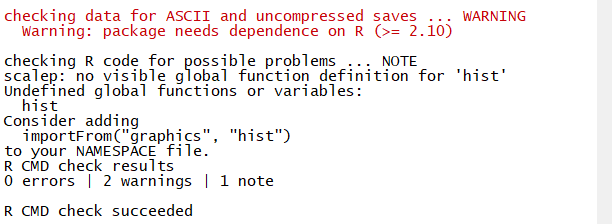
\includegraphics{images/testSS/autobuildresults.PNG}
\caption{}
\end{figure}

Although it's not necessary to understand every check that the check
function runs, it's worth noting that every check it performs is
relatively important, and if it signals any warnings or errors, it's
definitely worth fixing them. It's also probably worth fixing any
``notes'' it issues. If you're curious, you can read more about what
each type of check in the automated check does
\href{http://r-pkgs.had.co.nz/check.html\#check}{here}.

\subsection{Bonus: The goodpractice
Package}\label{bonus-the-goodpractice-package}

The aforementioned automated checking system for R is pretty good, but
there is a slightly more comprehensive version: the
\href{https://github.com/MangoTheCat/goodpractice/blob/master/vignettes/goodpractice.Rmd}{goodpractice
package}. The \texttt{goodpractice} package has an informative name -
the entire purpose of the package is to check whether your package
follows proper package development conventions and procedures
(i.e.~whether your package follows good practices). For example, running
the \texttt{goodpractice} package on the \texttt{devex} package yielded
the following helpful results:

\begin{figure}
\centering
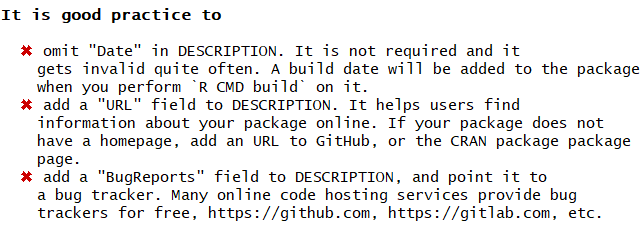
\includegraphics{images/testSS/goodpractice1.PNG}
\caption{}
\end{figure}

Let's run through the key points of using \texttt{goodpractice} below.

To install the goodpractice package, just run the following command in
the R console:

\begin{Shaded}
\begin{Highlighting}[]
\KeywordTok{install.packages}\NormalTok{(}\StringTok{'goodpractice'}\NormalTok{)}
\end{Highlighting}
\end{Shaded}

Once you've installed the \texttt{goodpractice} package, you basically
only need to use a single function from it: the \texttt{gp()} or
\texttt{goodpractice()} function (which call the same code). This
function will run comprehensive automated checks on your package, and it
takes exactly one input, the path of your built package. However, it's
important to note that the path of your \emph{built} package is not
identical to the path of the repo containing it. For example, I work on
the \texttt{devex} package in
``/Users/name/Documents/R/packageguidelines/devex'', but the built
package lives at another location. For \texttt{goodpractice()} to work,
you need to use this latter path. If you don't know what the path is,
you can use the ``system.file'' function to retrieve it for you, as
demonstrated below.

\begin{Shaded}
\begin{Highlighting}[]
\CommentTok{# Retrieve path}
\NormalTok{package_path <-}\StringTok{ }\KeywordTok{system.file}\NormalTok{(}\DataTypeTok{package =} \StringTok{'devex'}\NormalTok{)}

\CommentTok{# Check package}
\KeywordTok{library}\NormalTok{(goodpractice)}
\KeywordTok{gp}\NormalTok{(package_path)}
\end{Highlighting}
\end{Shaded}

And that's it! The \texttt{goodpractice} package is a bit picky, so it's
okay to leave a few concerns unresolved, but in general it gives good
advice. If you're diligent, you might eventually see a result like this:

\begin{figure}
\centering

\includegraphics{images/testSS/goodpractice2.PNG}
\caption{}
\end{figure}

which signals that your package conforms to all good practices. Lastly,
although it's beyond the scope of this guide, you ought to know that you
can create custom checks using the \texttt{goodpractice} package, as
documented
\href{https://github.com/MangoTheCat/goodpractice/blob/master/vignettes/custom_checks.Rmd}{here}.

\subsection{Tips and Tricks}\label{tips-and-tricks}

When testing, there are a couple of key principles to keep in mind:

\begin{enumerate}
\def\labelenumi{\arabic{enumi}.}
\tightlist
\item
  You want to expose bugs as quickly as possible so they don't create
  even larger headaches down the road! As Christopher Gandrud puts it,
  testing is all about `failing faster.' To this end, you should
  continuously test your packages.
\item
  Make sure your tests \emph{cover} the package code and also test all
  of the key functionality of the package. In an ideal world, a package
  should pass all of its tests only if all of its core functionality is
  bug-free.
\item
  Test names, organization, and error messages must be descriptive and
  easy to understand. One of the main purposes of tests is to inform you
  \emph{where} your code is failing, and to understand that, you need
  informative error messages. Otherwise, you will find yourself spending
  hours traversing your code to find bugs.
\end{enumerate}

The \texttt{devtools} cheatsheet, linked
\href{https://www.rstudio.com/wp-content/uploads/2015/03/devtools-cheatsheet.pdf}{here},
references a lot of the key components of the \texttt{testthat} package.

\section{Documentation}\label{documentation}

Documentation is an absolutely essential part of any package - most
people won't be willing to read your source code to figure out how your
functions work. Thankfully, creating documentation for your package is
incredibly easy with \texttt{Roxygen2}.

\subsection{Documenting Functions}\label{documenting-functions}

(Note: here, we describe how to document functions. For a more detailed
description of how to document S3, S4, and reference classes, check out
\href{http://r-pkgs.had.co.nz/man.html}{this page}.)

To understand how to use \texttt{Roxygen2}, it's best to start with an
example. Consider the following code, which generates the documentation
for the \texttt{general\_sqrt()} function above.

\begin{Shaded}
\begin{Highlighting}[]
\CommentTok{#' Generalized Square Roots}
\CommentTok{#'}
\CommentTok{#' \textbackslash{}code\{general_sqrt\} returns the square root of any real number}
\CommentTok{#'}
\CommentTok{#' @param x A real number - integers or doubles are both acceptable.}
\CommentTok{#' @return A complex value. If x is positive, the imaginary component is equal to 0;}
\CommentTok{#' if x is negative, the real component is equal to 0.}
\CommentTok{#'}
\CommentTok{#' @examples}
\CommentTok{#' general_sqrt(10)}
\CommentTok{#' general_sqrt(-10)}
\CommentTok{#' general_sqrt(-1)}
\CommentTok{#'}
\CommentTok{#' @export}
\CommentTok{# This function takes the complex square root of real numbers}

\NormalTok{general_sqrt <-}\StringTok{ }\ControlFlowTok{function}\NormalTok{ (x) \{}

  \CommentTok{# Return the normal square root if x > 0}
  \ControlFlowTok{if}\NormalTok{ (x }\OperatorTok{>}\StringTok{ }\DecValTok{0} \OperatorTok{||}\StringTok{ }\NormalTok{x }\OperatorTok{==}\StringTok{ }\DecValTok{0}\NormalTok{) \{}
    \KeywordTok{return}\NormalTok{(}\KeywordTok{complex}\NormalTok{(}\DataTypeTok{real=}\KeywordTok{sqrt}\NormalTok{(x), }\DataTypeTok{imaginary=}\DecValTok{0}\NormalTok{))}
\NormalTok{  \}}

  \CommentTok{# Else return the complex square root}

  \ControlFlowTok{else}\NormalTok{ \{}
    \KeywordTok{return}\NormalTok{(}\KeywordTok{complex}\NormalTok{(}\DataTypeTok{real =} \DecValTok{0}\NormalTok{, }\DataTypeTok{imaginary =} \KeywordTok{sqrt}\NormalTok{(}\OperatorTok{-}\NormalTok{x)))}
\NormalTok{  \}}

\NormalTok{\}}
\end{Highlighting}
\end{Shaded}

\begin{figure}
\centering
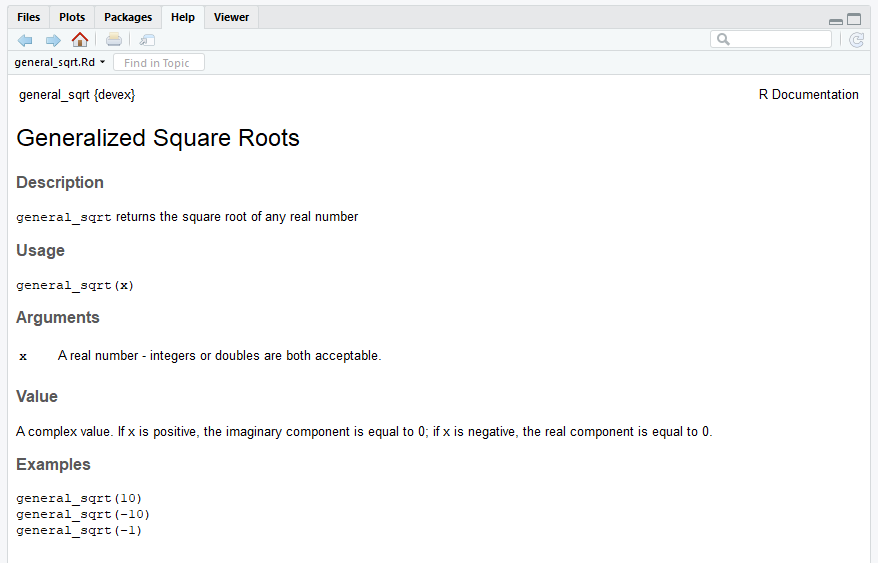
\includegraphics{images/packageSS/gensqrtdoc.PNG}
\caption{}
\end{figure}

Inside the R script, the documentation appears right above the
definition of the function - this is helpful because it will help you
remember to keep your documentations/functions up to date with each
other. Let's work through how this documentation was generated.

\begin{enumerate}
\def\labelenumi{\arabic{enumi}.}
\item
  Note that everything you write in \texttt{Roxygen2} should be preceded
  by a \#' character combo. This signals to the R environment that
  you're writing documentation, not code.
\item
  You should start your documentation with a very short (2-4 word) title
  of the function. In the example given above, the
  \texttt{general\_sqrt()} function is titled ``Generalized Square
  Roots.''
\item
  You should describe your functions' parameters using the
  `\citet{param}' signifier. This should succinctly describe the type
  (i.e.~double, integer, character) of the parameter, as well as its
  function, as well as any potential default value.
\item
  You should document the type of output your function returns. Is it an
  integer, a dataframe, a matrix? Does it depend on the input? Your
  documentation should answer these questions!
\item
  You \emph{must} provide examples of your function's use. These are
  pretty critical, because a lot of programmers will just skip straight
  to the examples (and only look at the rest of the documentation if the
  examples are unclear).
\item
  You may choose to write `\citet{export}' at the end of your
  documentation block. You should only do this if you want other people
  to use the function that you're exporting, because exporting it will
  make sure it shows up in the \textbf{namespace}, a document that makes
  sure your package works in combination with other packages. For
  example, if your package includes data labelled `lm', the namespace
  will prevent errors when using that data in combination with the R
  stats package (which has a function called `lm') and will \emph{not}
  throw an error. The
  \href{http://r-pkgs.had.co.nz/namespace.html}{exact mechanics of the
  namespace} are slightly beyond the scope of this guide, but thankfully
  \texttt{Roxygen2} will automatically generate a namespace for you when
  you create documentation with ``\citet{export}'' tags.
\end{enumerate}

Note that most functions you write won't be exported - for example, if
you write a helper function like \texttt{loss()} which is only used in
service of a larger function, it shouldn't be exported (exporting too
many functions `clutters' the namespace).

Once you've written all your documentation, it's fairly simple to check
what it looks like. Simply run the following function:

\begin{Shaded}
\begin{Highlighting}[]
\NormalTok{devtools}\OperatorTok{::}\KeywordTok{document}\NormalTok{()}
\end{Highlighting}
\end{Shaded}

which will automatically generate your documentation. Then, if you've
documented a function, you can type \texttt{?function-name} into the
console, and the documentation should automatically pop up!

After documenting your package, you can also click the `/man' folder to
inspect the documentation html files \texttt{Roxygen2} generates, but it
probably won't be more informative than simply typing
\texttt{?function-name} into the console.

\subsection{Adding a README}\label{adding-a-readme}

The README file is a bit different than the others, because your package
will actually work fine even if you don't have one. However, if you want
other people to use your package, it's best to have a README. The
purpose of a README is basically to bridge the gap between the
DESCRIPTION and the actual documentation in your package. In other
words, someone using your package might know what it does in a general
sense from your DESCRIPTION, but they won't necessarily know exactly how
to set up the package or how to use specific functions. The README takes
care of that. In general, READMEs should do at least two things, with a
couple of optional ones:

(Important):

\begin{enumerate}
\def\labelenumi{\arabic{enumi}.}
\tightlist
\item
  Offer a longer (one to three paragraph) description of the package,
  including core functions and bits and pieces of syntax
\item
  Help users install and set up the package
\end{enumerate}

(Optional from here on):

\begin{enumerate}
\def\labelenumi{\arabic{enumi}.}
\setcounter{enumi}{2}
\tightlist
\item
  Tell developers what to do if they want to contribute to your package
\item
  Help contributors figure out how to run the packages' unit tests
  (we'll talk more about unit tests in the next section)
\item
  Offer some acknowledgements
\end{enumerate}

This
\href{https://gist.github.com/PurpleBooth/109311bb0361f32d87a2}{template}
README is a good starting point. You could copy this file into your
package directory and modify it to reflect the content of your project.
Again, because your package will technically function without your
README, the actual structure and content of a README can be flexible.
However, just remember that if you don't have a README which outlines
why and how to use your package, other developers are unlikely to want
to use it.

\section{Vignettes}\label{vignettes}

Documentation is useful, but not necessarily a comprehensive guide to
your package. You may want to include details about your implementation,
extra examples, and more organization than your documentation provides,
which is exactly what vignettes are for.

\textbf{Vignettes} are basically articles which motivate and describe
your packages. They are generally written in RMarkdown, which allows you
to mix code, mathematical equations, and formatted text with ease. If
you are using RStudio, then writing vignettes will be very easy, because
RMarkdown works automatically with RStudio. On the other hand, if you
don't have RStudio, you will need to (i) run the
`install.packages(``rmarkdown'')' command, and (ii) install
\href{http://pandoc.org/installing.html}{pandoc}.

To write a vignette, start by running the \texttt{use\_vignette()}
function from the \texttt{usethis} package:

\begin{Shaded}
\begin{Highlighting}[]
\NormalTok{usethis}\OperatorTok{::}\KeywordTok{use_vignette}\NormalTok{(}\StringTok{'vignette-name'}\NormalTok{)}
\end{Highlighting}
\end{Shaded}

This function will create a `vignettes' subdirectory and populate it
with a file based on the name you specified. The file should look
something like this:

\begin{figure}
\centering
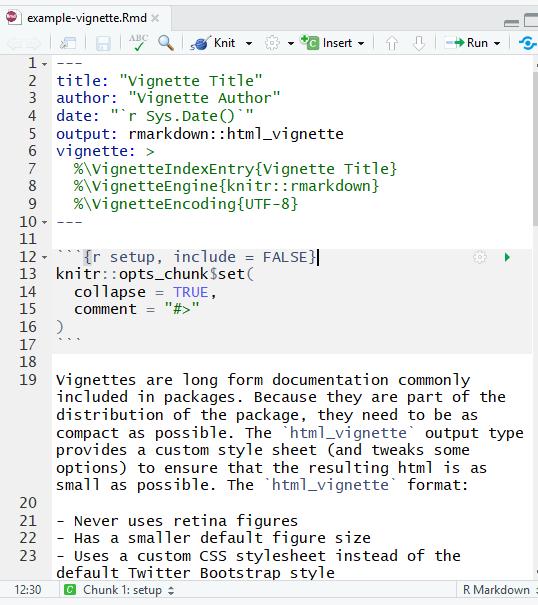
\includegraphics{images/packageSS/vignette1.PNG}
\caption{}
\end{figure}

The top of the file, between the two lines of dashes, is written in the
YAML language. It's simply a convenient way to specify metadata about a
vignette, and you should fill in the title and author fields.

The rest of the vignette should be written in RMarkdown, which is
basically a mix of Markdown, Latex, or code. The vignette template
generated by \texttt{usethis} \emph{is itself a guide to using
RMarkdown}, so we won't dive too deep into using RMarkdown. However,
there are a couple of core things you should know:

\begin{enumerate}
\def\labelenumi{\arabic{enumi}.}
\tightlist
\item
  By default, text in RMarkdown files is assumed to be written in
  \href{http://pandoc.org/MANUAL.html}{pandoc's flavor of Markdown}.
\item
  If you would like to include inline equations, you can do so by
  surrounding math symbols with a single dollar sign on each end. If
  you'd like to give an equation its own line, you can use two dollar
  signs on each end of the equations.
\end{enumerate}

\begin{figure}
\centering
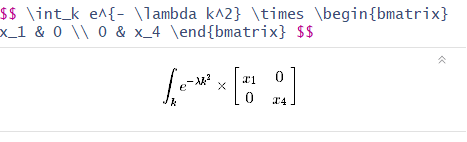
\includegraphics{images/packageSS/vignettemath.PNG}
\caption{\emph{Including math is easy in RMarkdown}}
\end{figure}

\begin{enumerate}
\def\labelenumi{\arabic{enumi}.}
\setcounter{enumi}{2}
\tightlist
\item
  You can add chunks of R code (and even other languages!) to your
  Vignette file by wrapping R code in `````'' symbols, as demonstrated
  below:
\end{enumerate}

\begin{figure}
\centering
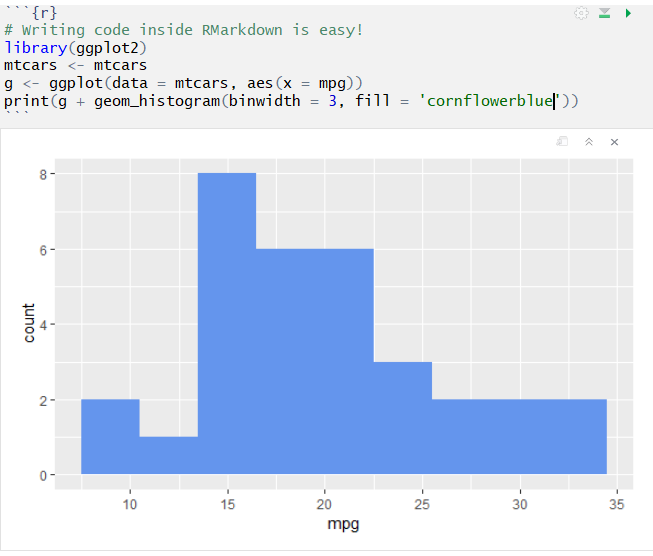
\includegraphics{images/packageSS/vignettecode.PNG}
\caption{}
\end{figure}

Once you've modified your vignette, you can \emph{knit} it into a
beautiful HTML document by running the following function in the
console:

\begin{Shaded}
\begin{Highlighting}[]
\NormalTok{rmarkdown}\OperatorTok{::}\KeywordTok{render}\NormalTok{(}\StringTok{'path/to/rmarkdown/file.Rmd'}\NormalTok{)}
\end{Highlighting}
\end{Shaded}

If you do choose to write vignettes, remember that it's critical to
motivate \emph{why} you wrote your package in the first place.
Additionally, you should structure the vignette so that it gives users
an impression of the overarching structure of the package itself
(i.e.~group and organize your functions!).

\section{Adding and Documenting Data}\label{adding-and-documenting-data}

Sometimes, you'll want to include data as part of your package, either
to serve as an example for users or because your functions need it to
work. This is totally optional - not all packages need to include data -
but can be useful, so let's walk through how to include (and document)
data in your package. Note that there are at least two kinds of data you
should think about including, but for both kinds of data, you should
generally save them as `.rdata' or `.rda' files (which are the same
thing).

\subsection{Including data which should be available to
users}\label{including-data-which-should-be-available-to-users}

All of the data you want to be available to users should be saved in a
folder called `data' inside your project. The way to do this is to write
and run a script which loads your data into R and then uses the
\texttt{usethis} function \texttt{use\_data()} to save it to a path
inside `data'. Even if you do not already have a folder called `data' in
your package, the \texttt{use\_data()} function will make it for you.
Note that for this to work, your working directory must be set to the
package you're writing, otherwise \texttt{usethis} won't know where to
put your data.

For example, when documenting the \texttt{scalep()} function, one might
want to include data as an example of a way to use \texttt{scalep()}. To
this end, we can use the built-in R dataset \texttt{mtcars} and include
it in the package.

\begin{Shaded}
\begin{Highlighting}[]
\NormalTok{usethis}\OperatorTok{::}\KeywordTok{use_data}\NormalTok{(mtcars)}
\end{Highlighting}
\end{Shaded}

In this way, you can include in your package any data you want,
providing it has been stored in an R object. Data in your `data' folder
will effectively always be exported, so you always must document it. To
document data, you should create an R Script in your `R' directory
called {[}`data.R'{]} and use \texttt{Roxygen2} to document the data
similarly to the way you'd document a function. For example, one might
document the aforementioned data in the following way:

\begin{Shaded}
\begin{Highlighting}[]
\CommentTok{#' Motor trend car road tests dataset}
\CommentTok{#'}
\CommentTok{#' This dataset lists the properties of 32 motorcars}
\CommentTok{#'}
\CommentTok{#' @format A dataframe with 32 rows and 11 columns.}
\CommentTok{#' \textbackslash{}describe\{}
\CommentTok{#'   \textbackslash{}item\{mpg\}\{Mile per gallon\}}
\CommentTok{#'   \textbackslash{}item\{cyl\}\{Number of cylinders\}}
\CommentTok{#'   \textbackslash{}item\{disp\}\{Displacement (cu.in)\}}
\CommentTok{#'   \textbackslash{}item\{hp\}\{Gross horsepower\}}
\CommentTok{#'   \textbackslash{}item\{drat\}\{Rear axle ratio\}}
\CommentTok{#'   \textbackslash{}item\{wt\}\{Weight (1000 lbs)\}}
\CommentTok{#'   \textbackslash{}item\{qsec\}\{1/4 mile time\}}
\CommentTok{#'   \textbackslash{}item\{vs\}\{Engine: (0 = V-shaped, 1 = straight)\}}
\CommentTok{#'   \textbackslash{}item\{am\}\{Transmission: (0 = automatic, 1 = manual)\}}
\CommentTok{#'   \textbackslash{}item\{gear\}\{Number of forward gears\}}
\CommentTok{#'   \textbackslash{}item\{carb\}\{Number of carburetors\}}
\CommentTok{#'\}}
\CommentTok{#' @source This dataset is a built-in R dataset and is}
\CommentTok{#' intended only to be used as an example for package development.}
\StringTok{"mtcars"}
\end{Highlighting}
\end{Shaded}

This should all look pretty similar to documenting functions. Note that
`\citet{format}' is a tag which will allow you to describe the structure
of a dataset, and it's good practice to list what each column measures
in this section. The `\citet{source}' section describes where the data
came from. Never write `\citet{export}' in this section, as data here is
already automatically exported.

\subsection{Including data for your
functions}\label{including-data-for-your-functions}

Some functions may rely on a large, predefined set of coefficients or
other inputs which need to be included in the package. However, users
shouldn't generally have access to such data because otherwise they
might accidentally radically change the way your function works. It's
best to put such data in `R/sysdata.rda', because then users won't
easily be able to access and accidentally modify it. As before, the way
to include data in this way is to write a script which loads the data
into R and then use the \texttt{use\_data()} function to save it, but
you should also include a parameter \texttt{internal\ =\ TRUE} in the
function call to let R know that this is interior, not exterior, data.
For example, if a function depends on a matrix called ``coefficients'',
one might run the following code:

\begin{Shaded}
\begin{Highlighting}[]
\NormalTok{coefficients <-}\StringTok{ }\KeywordTok{read.csv}\NormalTok{(}\StringTok{'Users/name/Documents/R/coefs.csv'}\NormalTok{)}
\NormalTok{usethis}\OperatorTok{::}\KeywordTok{use_data}\NormalTok{(coefficients, }\DataTypeTok{internal =} \OtherTok{TRUE}\NormalTok{)}
\end{Highlighting}
\end{Shaded}

Data in `R/sysdata.rda' is never exported, so there's no need to
document it.

\hypertarget{releasing-your-package}{\section{Releasing Your
Package}\label{releasing-your-package}}

You're almost done at this point! You've written your functions,
modified the description, documented your functions, presumably exported
some of them, and hopefully tested all of them; you're now ready to
\emph{release} and \emph{publicize} your package. There are basically
two main ways to do this.

\subsection{Pushing to GitHub}\label{pushing-to-github}

The easiest way to publish your package is to simply
\href{./version-control}{push it to GitHub}, (we'll discuss how to do
this later). The pros of this approach are that it makes it very easy
for users to download your package - they can literally do it in one
line. Additionally, Github offers free services
\href{https://pages.github.com/}{to host a website for your package and
its documentation}, and most importantly, it's very easy for
\textbf{you} to publish your package this way. Thus, pushing to Github
is sort of the ``default'' way to publish a smaller package.

\subsection{CRAN}\label{cran}

On the other hand, if you've written a larger package which you would
like to distribute to the entire R community, you might consider
submitting it to \href{https://cran.r-project.org/}{CRAN}, the
Comprehensive R Archive Network. CRAN is basically the official package
authority designated by the R community, and successfully adding your
package to CRAN will make it more legitimate as well as easier for R
users to find and install.

Logistically, submitting your package to CRAN is pretty simple. The
first step is to \textbf{build} your package, which means bundling it
into a format that is easy to distribute and easy for users to install.

The best way to build your package is to zip it as a .tar.gz file.
\texttt{devtools} will do this for you if you run the following command:

\begin{Shaded}
\begin{Highlighting}[]
\NormalTok{devtools}\OperatorTok{::}\KeywordTok{build}\NormalTok{(}\DataTypeTok{binary =} \OtherTok{FALSE}\NormalTok{)}
\end{Highlighting}
\end{Shaded}

and then you should see a tar.gz file pop up just outside your working
directory.

The next step is to submit the bundled file to CRAN
\href{https://cran.r-project.org/submit.html}{at the link here}, along
with a couple of comments. Although this seems pretty simple, in
actuality, CRAN has very high standards for packages, so it can be
rather tricky to get a package accepted. CRAN's specific standards are
beyond the scope of the current iteration of this guide, but if you
decide you want to publish a package on CRAN, you should read
\href{http://r-pkgs.had.co.nz/release.html}{Hadley Wickham's advice on
the subject} \textbf{very carefully.}

\subsubsection{Optional: Building precompiled
binaries}\label{optional-building-precompiled-binaries}

tar.gz files are useful because anyone who has a working R development
environment can install and unzip your package, regardless of their
operating system. However, you do need a development environment to
install packages built as tar.gz files, and some users (in particular on
Windows) may not have development environments set up yet. To address
this potential issue, another way to build your package is as a
\textbf{precompiled binary file}. Precompiled binaries are useful
because unlike tar.gz files, they do not require a development
environment to install. However, they are platform specific: a
precompiled binary built by a Windows machine can't be installed on Mac
machine. Although tar.gz files are much more common, if you do want to
build a binary, you can just change an argument of
\texttt{devtools::build()}:

\begin{Shaded}
\begin{Highlighting}[]
\NormalTok{devtools}\OperatorTok{::}\KeywordTok{build}\NormalTok{(}\DataTypeTok{binary =} \OtherTok{TRUE}\NormalTok{)}
\end{Highlighting}
\end{Shaded}

and your precompiled binary will be built.

\subsection{Publicizing}\label{publicizing}

Once you've released your package either on Github or perhaps on CRAN,
you should publicize it! You can of course publicize it any way you
choose, but there are at least two things you should consider doing.

\begin{enumerate}
\def\labelenumi{\arabic{enumi}.}
\tightlist
\item
  Tweet about your package using the \#rstats hashtag, which reaches a
  substantial portion of the R community.
\item
  You may also want to send an email out to the
  \href{https://stat.ethz.ch/mailman/listinfo/r-packages}{R-Packages
  email list}.
\end{enumerate}

And that's it!

\section{Tips and Tricks}\label{tips-and-tricks-1}

First, there's a wonderful cheat sheet for package development linked
\href{https://www.rstudio.com/wp-content/uploads/2015/06/devtools-cheatsheet.pdf}{here}.

Second, if you're having trouble, you can always just reference
\href{https://stackoverflow.com/questions/tagged/r}{stackoverflow}.

\chapter{Version Control}\label{version-control}

\textbf{Version Control} is the process of organizing and sharing
different versions of your code, and it's surprisingly important. This
chapter is a beginner-friendly introduction to Version Control with Git
and GitHub. In it, we'll motivate Git/GitHub, and then discuss what
precisely Git/GitHub do and how to use them.

There are other tools for Version Control out there, but Git/GitHub are
by far the most common, so we've chosen to focus on them. As you might
expect, much (but not all) of the logic behind GitHub applies to other
version control systems too.

\section{Why use Git/GitHub?}\label{why-use-gitgithub}

Git and GitHub are actually two different things, and deserve their own
sections. Before diving into specifics, however, we should talk about
why Git/GitHub exist in the first place. Broadly, Git and GitHub are
just tools that developers use to organize their code, which
specifically solve three main organizational problems.

First, imagine that two imaginary programmers named Carlos and Grace are
working together to build a website that automatically displays polling
results from US elections, and suppose Grace modifies a script to change
the method for aggregating polling data. It would be tedious for Carlos
and Grace to email the script back and forth each time they updated it.
Instead, they need a \emph{repository} where they can update and sync
their code to make sure they're on the same page. GitHub allows
programmers to create such repositories.

Second, imagine that farther along in the project, Grace decides that
she needs to totally rewrite the code which stores and organizes polling
data. Unfortunately, while Grace modifies the system which stores the
data, it will be offline, which is unfortunate because Carlos needs to
use the data for his work on the project. To avoid this dilemma, Git and
GitHub allow programmers to create different versions, called
\emph{branches}, of their code. By branching, Grace can modify the
storage system, and in the meantime, Carlos can continue to use the old
storage system for his work.

Third, suppose that once Grace and Carlos have finished their website,
they want to publish all the statistical functions and tools they built
so that other researchers can use those tools to reproduce Grace and
Carlos's research. Putting all of their work on GitHub is probably the
quickest and easiest way to make it accessible to other researchers.

\subsection{What is Git?}\label{what-is-git}

\begin{figure}
\centering
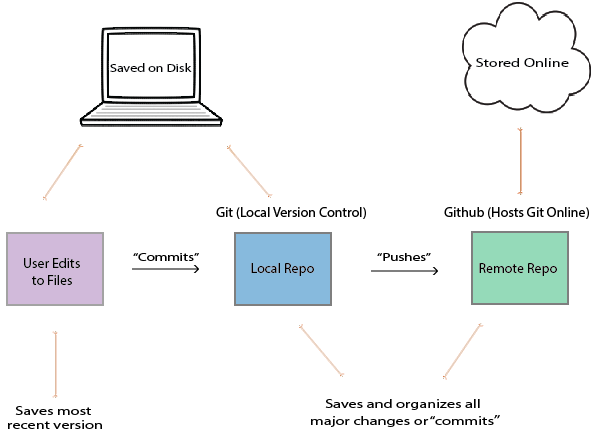
\includegraphics{images/gitgraphic.PNG}
\caption{}
\end{figure}

Git is a local version control system. In other words, Git automatically
organizes and saves versions of code on your computer, but does not
connect to the internet: it's purely accessible through the command
prompt on a computer (there are also other ways to use Git, but it's
generally best to use the command prompt). Git organizes code in two
ways.

First, Git sends discrete versions of code to a local database or
repository on the computer on which it is installed. To understand this,
imagine that Carlos is writing an R script which determines the proper
weights for aggregating polling data, and at some point he finishes the
first version of the script. At this point, Carlos can send his code to
the local repository, in an action called \emph{commiting} his script.
We'll discuss how to do this later, but note that scripts are not
automatically committed to the repository. If Carlos deleted all the
code in the script and saved it, he could still access the script by
going into the repository. Moreover, the repository also stores all of
the previous versions of code, and can backtrack through the various
commits, so if Carlos decides the version of the script he built last
year worked better, he can use Git to access it.

Second, Git can create branches, or separate versions of code, on the
computer it's installed to. Remember how Grace wanted to revamp the
storage system for polling data without preventing Carlos from accessing
the old storage system? Using Git, Grace should create a new
\emph{branch} in the repository. For most practical purposes, each
branch exists as a separate version of the entire polling project in the
Git repository, allowing Grace to modify and experiment without
compromising the functionality of the \emph{master} or original branch.

While she's working, Grace can use Git to move back and forth between
the branches. Then, when she finishes designing and testing the new
storage system, she can \emph{merge} the two branches together, and
Carlos's scripts will automatically start using the new storage system.

\subsection{What is GitHub?}\label{what-is-github}

Where Git creates \emph{local} repositories on an individual computer,
GitHub allows programmers to create \emph{remote} repositories, stored
online, for their code. This is a pretty simple concept, but it's
extroardinarily useful. It means that when Grace finishes updating a
series of scripts, she can simply \emph{push} (push means send) them to
GitHub, and then Carlos can in one command \emph{pull} (download) the
modified versions onto his computer to work with them. GitHub provides
other important tools, but we will not discuss those until later.

\section{Setting up Git/GitHub}\label{setting-up-gitgithub}

\subsection{Making a GitHub account}\label{making-a-github-account}

Signing up for a GitHub is fairly simple - just go to GitHub.com, click
``sign up'' in the upper right hand corner, and follow the instructions.
We recommend, at least to begin with, getting a free version of GitHub.

\subsection{How to Install and Set Up
Git}\label{how-to-install-and-set-up-git}

Because Git is a form of \emph{local} source control, it does require
installation. To install Git onto your computer, go to one of the
following sites:

\begin{itemize}
\item
  For Linux: Head to \url{https://git-scm.com/download/linux} and follow
  the instructions.
\item
  For Windows: Go to \url{https://git-scm.com/download/win} and the
  download should automatically start.
\item
  For Mac: Click on \url{https://git-scm.com/download/mac} and the
  download should automatically start.
\end{itemize}

If you are running Windows/Mac and the websites above download an
installer, simply follow the instructions from the installer - it's fine
to just use default settings.

Before you can start using Git, you do have to do a one time set up. Git
is built to track and organize old versions of code, so it will need you
to set your username and email before it will let you start modifying
programs. To set your username and email after installing, open the
command line on your computer and type the following commands into it:

\begin{Shaded}
\begin{Highlighting}[]
\OperatorTok{$}\StringTok{ }\NormalTok{git config }\OperatorTok{--}\NormalTok{global user.name }\StringTok{"Your Name"}
\OperatorTok{$}\StringTok{ }\NormalTok{git config }\OperatorTok{--}\NormalTok{global user.email }\StringTok{"youremail@email.com"}
\end{Highlighting}
\end{Shaded}

You might not get explicit confirmation from the command line - for
example, when I set the username/email, I see the image below - but
don't worry, Git has still received the message.

\begin{figure}
\centering
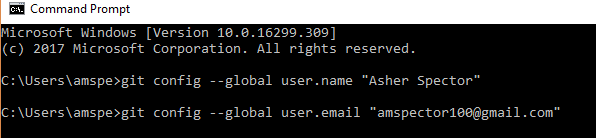
\includegraphics{images/configglobals.PNG}
\caption{}
\end{figure}

Now you're ready to start using Git/GitHub!

\section{Using Git/GitHub}\label{using-gitgithub}

\subsection{Initializing Projects and
Repositories}\label{initializing-projects-and-repositories}

The first step to using Git is creating a project, or repository (repo
for short). To do so, log into your GitHub account. Look near the
top-right for your profile icon, click it, and click ``Your Profile.''
Then you should see ``Repositories'' in the top tab, and click on
``Repositories''. Then click the green ``New'' button on the right.

\begin{figure}
\centering
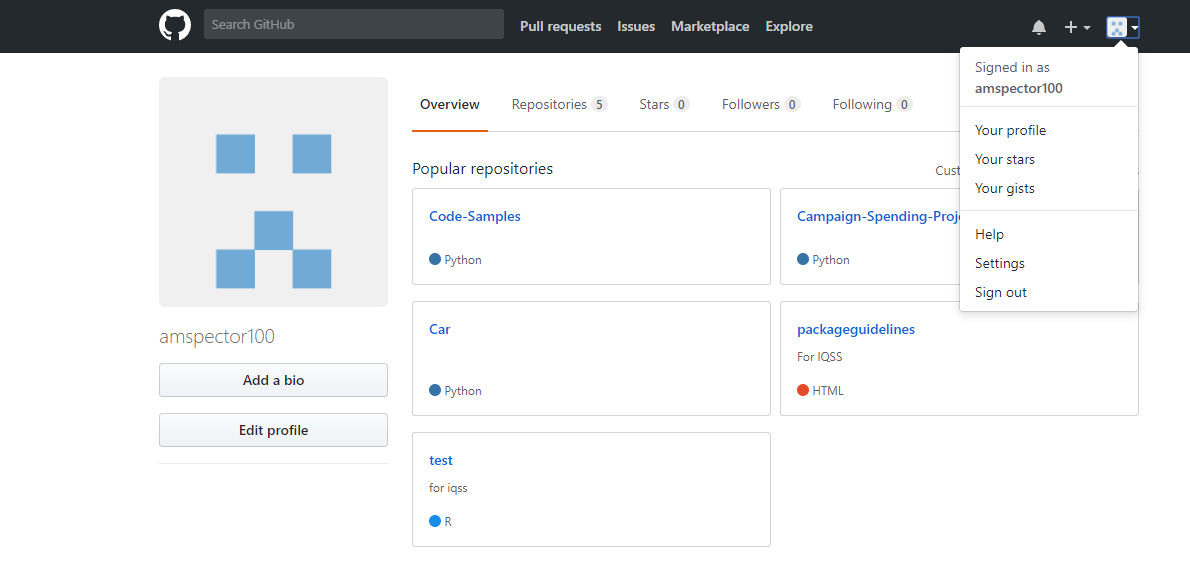
\includegraphics{images/gitdashboard.PNG}
\caption{}
\end{figure}

GitHub will prompt you to choose a repository name and description of
the repo, which you should enter, and will also ask you whether you'd
like to initialize the repository with a README, a .gitignore file, and
a license. For now, just initialize the repo with the README file.

Once you've created the repository on GitHub, the next step is to link
it with a local Git repository. To do this, open the \emph{command
prompt} on your computer. You'll need to enter a couple of commands to
get the repo set up on your computer.

First, you'll need to set the \emph{working directory} in the command
prompt. The working directory is the location where Git and command
prompt will execute all of your commands - ie. if you tell Git to create
a new file, the new file will be located your working directory. Thus,
before you download your repository, you'll want to navigate to the
folder in which you want the repository to be located. For example,
Carlos might want to put a repo in his ``R'' folder inside the
``Documents'' folder on his computer. To do this, he'd use the
\texttt{cd} command, which stands for ``change directory,'' and then
copy and paste the path of the folder he'd like to place the repository
in. An example is given below:

\begin{Shaded}
\begin{Highlighting}[]
\OperatorTok{$}\StringTok{ }\NormalTok{cd }\OperatorTok{~}\ErrorTok{/}\NormalTok{Documents}\OperatorTok{/}\NormalTok{R}
\end{Highlighting}
\end{Shaded}

Next, you will need to tell Git to download, or \emph{clone}, the repo.
You can do this using the \texttt{git\ clone} command, which allows you
to download and sync a repository \emph{for the first time.} This will
download the repo, with all its contents, onto your computer and
automatically set up a local version of the repo. See an example of the
command below:

\begin{Shaded}
\begin{Highlighting}[]
\OperatorTok{$}\StringTok{ }\NormalTok{git clone https}\OperatorTok{:}\ErrorTok{//}\NormalTok{GitHub.com}\OperatorTok{/}\NormalTok{Carlos_Account}\OperatorTok{/}\NormalTok{repository_name}\OperatorTok{/}
\end{Highlighting}
\end{Shaded}

\subsection{Modifying Projects}\label{modifying-projects}

It's best practice to create new R code files in your local project
repository. When you save your code files, initially git will not be
aware of them - that is, they will not be \emph{tracked}, but we can
change this by \emph{adding} them to the local repository using the
command \texttt{git\ add\ .}. Here, the period following
\texttt{git\ add} tells Git that we want to start tracking all the files
in the directory.

\begin{Shaded}
\begin{Highlighting}[]
\OperatorTok{$}\StringTok{ }\NormalTok{cd }\OperatorTok{~}\ErrorTok{/}\NormalTok{Documents}\OperatorTok{/}\NormalTok{R}\OperatorTok{/}\NormalTok{repository_name}
\OperatorTok{$}\StringTok{ }\NormalTok{git add .}
\end{Highlighting}
\end{Shaded}

Once new files are being tracked, we can put them under version control
by \emph{commiting} them, using the command \texttt{git\ commit}. You
can add a message to indicate the changes you've made by typing
\texttt{git\ commit\ -m\ "\textless{}message-here\textgreater{}"}
followed by your message in quotes.

\begin{Shaded}
\begin{Highlighting}[]
\OperatorTok{$}\StringTok{ }\NormalTok{cd }\OperatorTok{~}\ErrorTok{/}\NormalTok{Documents}\OperatorTok{/}\NormalTok{R}\OperatorTok{/}\NormalTok{repository_name}
\OperatorTok{$}\StringTok{ }\NormalTok{git commit }\OperatorTok{-}\NormalTok{m }\StringTok{"Fixed small bug"}
\end{Highlighting}
\end{Shaded}

Lastly, you need to \emph{push} the files, which means sending them to
GitHub online. You can do this by writing
\texttt{git\ push\ origin\ master}, which will send the file to the
remote GitHub repo.

\begin{Shaded}
\begin{Highlighting}[]
\OperatorTok{$}\StringTok{ }\NormalTok{git push origin master}
\end{Highlighting}
\end{Shaded}

If you move new files into your local repository, they will need to be
tracked using \texttt{git\ add\ .} and then committed using
\texttt{git\ commit\ -m\ "\textless{}message-here\textgreater{}"} before
they are under version control.

\subsection{Accessing older versions of
code}\label{accessing-older-versions-of-code}

You should never be scared of Git/GitHub, because they only add
information - they almost never delete it. In practice, this means that
if you commit horrible changes to your code, you can easily revert to a
previous version. For example, let's say Grace wrote some new functions
for a script, deleted them and committed the deletes later on, but now
wants the functions back. She can easily access the older script using
Git. First, she should use the \texttt{git\ log} command to see what
commits have been made recently.

\begin{Shaded}
\begin{Highlighting}[]
\OperatorTok{$}\StringTok{ }\NormalTok{git log}
\end{Highlighting}
\end{Shaded}

This command might give an output like this:

\begin{Shaded}
\begin{Highlighting}[]
\NormalTok{commit 06c347sa (HEAD ->}\StringTok{ }\NormalTok{master, origin}\OperatorTok{/}\NormalTok{master, origin}\OperatorTok{/}\NormalTok{HEAD)}
\NormalTok{Author}\OperatorTok{:}\StringTok{ }\NormalTok{Grace Smith }\OperatorTok{<}\NormalTok{gracesmith}\OperatorTok{@}\NormalTok{gmail.com}\OperatorTok{>}
\NormalTok{Date}\OperatorTok{:}\StringTok{   }\NormalTok{Sun Feb }\DecValTok{18} \DecValTok{23}\OperatorTok{:}\DecValTok{13}\OperatorTok{:}\DecValTok{32} \DecValTok{2018} \OperatorTok{-}\DecValTok{0500}

\NormalTok{    Remove storage functions}

\NormalTok{commit b69a14b}
\NormalTok{Author}\OperatorTok{:}\StringTok{ }\NormalTok{Grace Smith }\OperatorTok{<}\NormalTok{gracesmith}\OperatorTok{@}\NormalTok{gmail.com}\OperatorTok{>}
\NormalTok{Date}\OperatorTok{:}\StringTok{   }\NormalTok{Sat Feb }\DecValTok{17} \DecValTok{23}\OperatorTok{:}\DecValTok{11}\OperatorTok{:}\DecValTok{28} \DecValTok{2018} \OperatorTok{-}\DecValTok{0500}

\NormalTok{    Add storage functions}

\NormalTok{commit 8a237d1}
\NormalTok{Author}\OperatorTok{:}\StringTok{ }\NormalTok{Grace Smith }\OperatorTok{<}\NormalTok{gracesmith}\OperatorTok{@}\NormalTok{gmail.com}\OperatorTok{>}
\NormalTok{Date}\OperatorTok{:}\StringTok{   }\NormalTok{Fri Feb }\DecValTok{16} \DecValTok{21}\OperatorTok{:}\DecValTok{28}\OperatorTok{:}\DecValTok{46} \DecValTok{2018} \OperatorTok{-}\DecValTok{0500}

\NormalTok{    Initial commit}
\end{Highlighting}
\end{Shaded}

Clearly, Grace should restore the second commit listed, named `b69a14b,'
in order to access the functions she deleted. There are generally two
situations:

\begin{enumerate}
\def\labelenumi{\arabic{enumi}.}
\item
  If the changes have not been pushed onto the remote repository, to
  access the deleted functions, Grace can use the \texttt{git\ reset}
  command with the \texttt{-\/-hard} option and the commit number:
  \texttt{git\ reset\ -\/-hard\ b69a14b}. This will update the current
  version of the script to the \texttt{b69a14b} version, which Grace can
  then inspect and test until she's ready to commit it to Git/GitHub.
  Note that this is a pretty serious action to take because it will
  effectively delete all the commits after the version being restored.
\item
  If the changes have been pushed onto the remote repository, Grace can
  access the deleted functions using the following commands:
\end{enumerate}

\begin{Shaded}
\begin{Highlighting}[]
\OperatorTok{$}\StringTok{ }\NormalTok{git revert }\OperatorTok{--}\NormalTok{no}\OperatorTok{-}\NormalTok{commit head}
\OperatorTok{$}\StringTok{ }\NormalTok{git commit }\OperatorTok{-}\NormalTok{m }\StringTok{"<message-here>"}
\end{Highlighting}
\end{Shaded}

This will update the current version of the script to the
\texttt{b69a14b} version in Grace's local repository. Then Grace can
push it onto the remote repository using
\texttt{git\ push\ origin\ master} command.

\subsection{The .gitignore file}\label{the-.gitignore-file}

There's one more thing you should know about adding/modifying files that
will make your life a lot easier. Sometimes, when modifying and
commiting projects, you won't want to type out every individual file
you've modified: you'll instead want to use the \texttt{git\ add\ .}
command which will simply queue every modified file to be committed.

\begin{Shaded}
\begin{Highlighting}[]
\OperatorTok{$}\StringTok{ }\NormalTok{git add .}
\OperatorTok{$}\StringTok{ }\NormalTok{git commit }\OperatorTok{-}\NormalTok{m }\StringTok{"<message-here>"}
\OperatorTok{$}\StringTok{ }\NormalTok{git push}
\end{Highlighting}
\end{Shaded}

However, often, you'll have files in your directory which you do not
want to commit or push to GitHub because they'll clutter up the
directory. For example, R directories create ``.RHistory'' and
``.RData'' files which will save your history and working environment.
These are useful perhaps when writing code, but you don't want them
taking up space in your final packaged product.

To solve this problem, you can use a \emph{.gitignore file.} A
.gitignore file tells Git to ignore certain kinds of files when you
write \texttt{git\ add\ .}. For example, gitignore files are frequently
configured to tell git to ignore csv files, .RData files, installer
logs, and more.

Let's discuss how \emph{.gitignore} files actually work. A .gitignore
file is really just a glorified text file. However, its filename should
be just `.gitignore', because that's how Git recognizes it - then, if
you put a file titled `.gitignore' in a directory you're working on, Git
will use the .gitignore file to decide what to ignore in that specific
directory. For example, if Grace is working on a project in
`\textasciitilde{}/Documents/R/repo\_name', she should create a
`.gitignore' file inside that folder.

This still leaves an important question - how does Git use the
.gitignore file to determine which files to ignore? Essentially,
.gitignore files are just a bunch of independent lines of text, and each
line tells git another specific pattern of filepath to ignore. For
example, consider the following example of a .gitignore file:

\begin{figure}
\centering
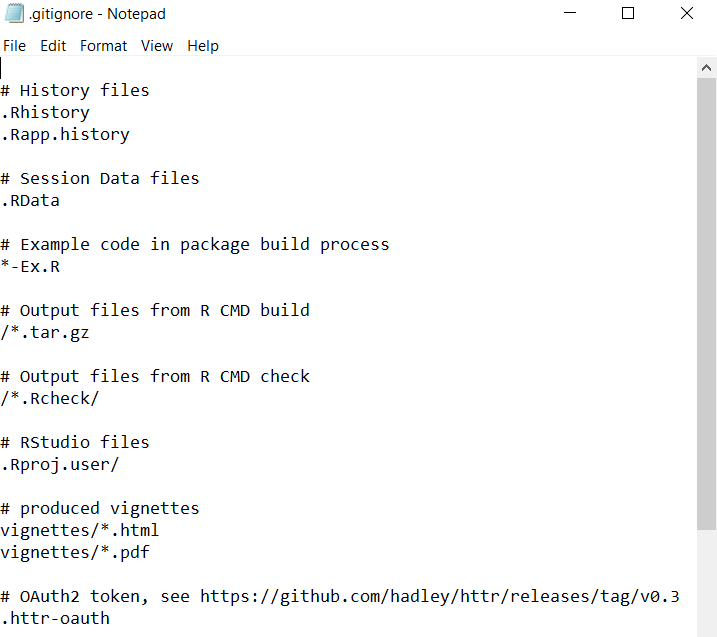
\includegraphics{images/gitignore3.PNG}
\caption{}
\end{figure}

Each line beginning with a \texttt{\#} is just a comment explaining the
function of that part of the .gitignore file. However, there are a
couple basic syntactical rules you need to understand.

\begin{enumerate}
\def\labelenumi{\arabic{enumi}.}
\item
  If you write `.filetype', then all files which end with `.filetype'
  will be ignored by git. For example, the third line in the above
  example reads `.RHistory', so all files with a `.RHistory' in the file
  name (even if the files are in subdirectories) will be ignored.
\item
  If you write `string', then everything in the directory which contains
  that `string' in it will be ignored. For example, if Grace wrote `dog'
  in her .gitignore, then git would ignore both a file called `dog.csv'
  and every file in a subdirectory called `dog'.
\item
  If you prepend a pattern with an asterisk *, then the asterisk *
  serves as a wildcard which can match 0 or more characters. For
  example, if I write ``*car``, then git will ignore the file `mycar.R'.
\item
  If you prepend a pattern with a forward slash `/', then git will only
  ignore files which match that pattern in the parent (root) directory.
  For example, I might write `/.csv' in my gitignore file. This would
  cause git to ignore a file with the path `dog.csv', but it would not
  ignore a file called `data/dog.csv'.
\item
  If you prepend a pattern with an exclamation mark, git will \emph{not}
  ignore that pattern. For example, if Grace really wanted to make sure
  her pictures of her dog were pushed to Git, she might write `!dog.PNG'
  to ensure git did not ignore that picture.
\end{enumerate}

The rules can seem confusing at times, but it's hard to go wrong -
usually, there are at least 10 ways to ignore any given file you want to
ignore. Moreover, if you're still confused, you might visit Atlassian,
which has a wonderful table of all of the various syntactical tricks you
can use in your own gitignores, linked
\href{https://www.atlassian.com/git/tutorials/gitignore}{here}.

Lastly (and most importantly), to save you time, the wonderful
\href{https://www.iq.harvard.edu/people/nalette-brodnax}{NaLette
Brodnax} has created a template .gitignore file which you can use to
declutter your GitHub repos. Using it requires three steps:

Step 1: Download the file `template.gitignore' from
\href{https://github.com/IQSS/Rbuild/blob/master/template.gitignore}{here}.
It should look something like this when you open it:

\begin{figure}
\centering
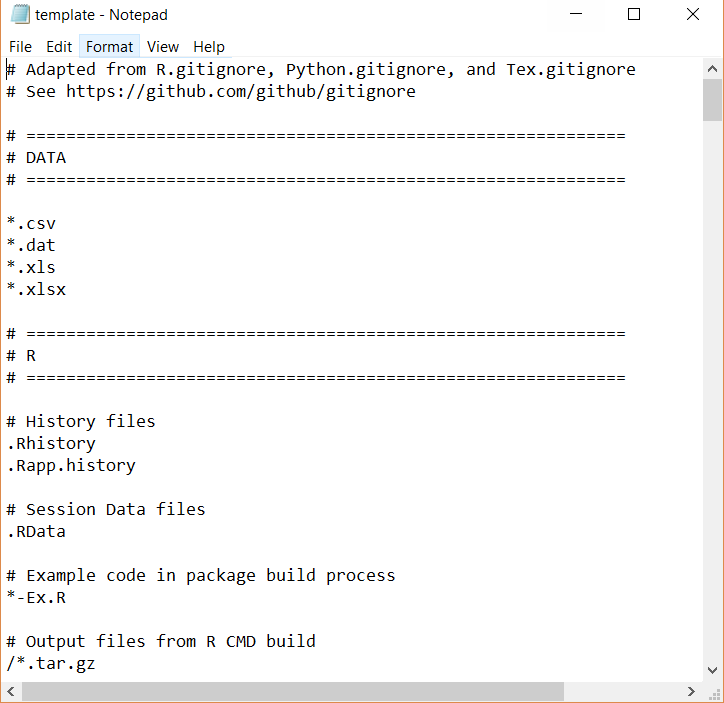
\includegraphics{images/gitignore.PNG}
\caption{}
\end{figure}

Step 2: Manually move the template file from your downloads folder to
the directory of interest. For example, if Grace is working on a project
in `\textasciitilde{}/Documents/R/repo\_name', she should copy the
template into that folder.

Step 3: Open the `template.gitignore' file in the folder and save it
just as `.gitignore'. This will help git recognize that your .gitignore
file is in fact a .gitignore file. Your operating system might protest
at this - Windows in particular freaks out at `.gitignore' files, which
is why we initially named the template `templates.gitignore' instead of
just `.gitignore'. However, once the .gitignore file is in the correct
directory, it's safe to change the path. Your end result should look
something like this:

\begin{figure}
\centering

\includegraphics{images/gitignore2.PNG}
\caption{A .gitignore file}
\end{figure}

It has no name, but it will serve its intended purpose.

If you decide to create your own .gitignore file, you can follow very
similar steps.

\begin{enumerate}
\def\labelenumi{\arabic{enumi}.}
\item
  Go into the directory you want and create a blank text file called
  `template.gitignore'. It's necessary at first to keep the `template'
  part because otherwise some operating systems will not let you create
  the file.
\item
  Start writing your gitignore file.
\item
  Save the file as `.gitignore.'
\end{enumerate}

.gitignore files aren't glamorous, but they really are important -
nobody wants to work with cluttered repositories.

\subsection{Branching}\label{branching}

\begin{figure}
\centering
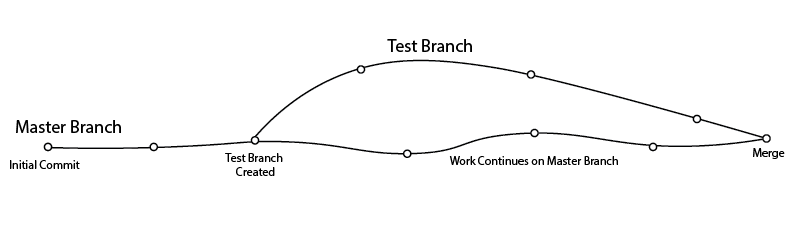
\includegraphics{images/branchinggraphic.PNG}
\caption{}
\end{figure}

As we discussed earlier, branches allow you to modify scripts while
simultaneous keeping the old versions easily accessible. In practice,
the way this works is that the branch you select in git changes the
appearance of the directory structure and files therein, when viewed in
explorer/finder. For example, if Carlos has the following script as the
master (default) branch in Git, the script might look something like
this when he opens it on his computer:

\begin{figure}
\centering
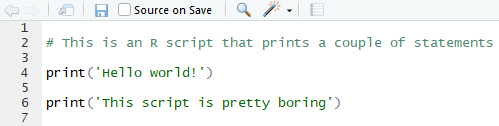
\includegraphics{images/hello1.PNG}
\caption{\emph{Master Branch of the Hello World Script}}
\end{figure}

However, if he uses Git to switch to a test branch, he might open the
exact same file using his file explorer and see the following:

\begin{figure}
\centering
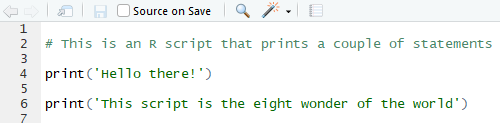
\includegraphics{images/hello2.PNG}
\caption{\emph{Test Branch of the Hello World Script}}
\end{figure}

Let's discuss how to actually use Git to branch.

\paragraph{Creating and Switching
Branches}\label{creating-and-switching-branches}

To create a branch, use the \texttt{git\ checkout} command followed with
a \texttt{-b} and the name of the branch:

\begin{Shaded}
\begin{Highlighting}[]
\OperatorTok{$}\StringTok{ }\NormalTok{git checkout }\OperatorTok{-}\NormalTok{b branch_name}
\end{Highlighting}
\end{Shaded}

This will create a new branch which is identical to the initial (master)
branch. You can modify it as you like, and you will still be able to
easily access the initial (master) branch. To do this, simply use the
\texttt{git\ checkout} command without the \texttt{-b} and type the name
of the branch you want to switch to:

\begin{Shaded}
\begin{Highlighting}[]
\OperatorTok{$}\StringTok{ }\NormalTok{git checkout switch_to_this_branch}
\end{Highlighting}
\end{Shaded}

Remember, switching to a branch will change the way the file shows up
once you open it from your computer.

\paragraph{Merging Branches}\label{merging-branches}

Suppose you have created a test branch, tested it to make sure it works,
and now want to combine it with the original master branch. To do this,
use the \texttt{git\ checkout} command in combination with the
\texttt{git\ merge} command as follows:

\begin{Shaded}
\begin{Highlighting}[]
\OperatorTok{$}\StringTok{ }\NormalTok{git checkout master}
\OperatorTok{$}\StringTok{ }\NormalTok{git merge test_branch_name}
\end{Highlighting}
\end{Shaded}

These two commands will merge the test branch into the master branch,
meaning that the master branch at the end of the merging will look like
the test branch.

\subsection{Conflicts}\label{conflicts}

Sometimes Git will be unable to push or pull branches because it is
getting conflicting information from two users. For example, suppose
Grace has written the following function, which calculates the squared
error between two values:

\begin{figure}
\centering
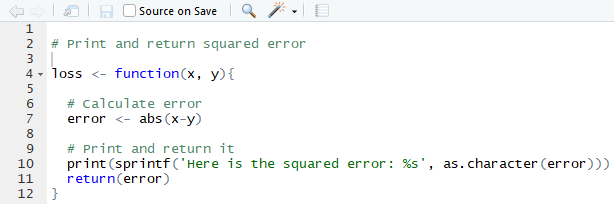
\includegraphics{images/loss0.PNG}
\caption{\emph{Original Version of Loss Script}}
\end{figure}

This function clearly has a bug in it, because it claims to return the
squared error, but instead, it returns the absolute value of the error.
Carlos notices this, and modifies the function so that it accurately
reports that it calculates the absolute value, and pushes his modified
version to GitHub:

\begin{figure}
\centering
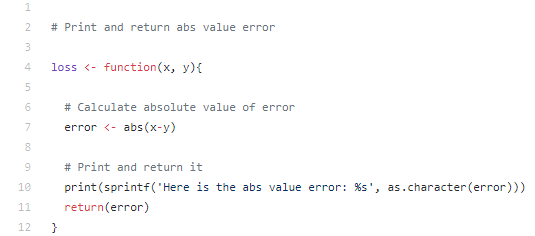
\includegraphics{images/lossCarlos.PNG}
\caption{\emph{Carlos's Pushed Version of Loss Script}}
\end{figure}

But before Grace realizes Carlos has modified the script, she also fixes
the bug, but instead by changing the absolute value to a squaring
function:

\begin{figure}
\centering
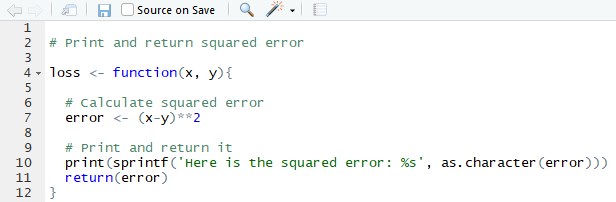
\includegraphics{images/lossGrace.PNG}
\caption{\emph{Grace's Modified Version of Loss Script}}
\end{figure}

Git is smart, so when Grace tries to push her version to GitHub, Git
will recognize that the two versions of the script conflict. As a
result, it will throw the following error:

\begin{Shaded}
\begin{Highlighting}[]
\NormalTok{C}\OperatorTok{:}\NormalTok{\textbackslash{}Users\textbackslash{}gracesmith\textbackslash{}Documents\textbackslash{}R\textbackslash{}repo_name}\OperatorTok{>}\NormalTok{git push}
\NormalTok{To https}\OperatorTok{:}\ErrorTok{//}\NormalTok{GitHub.com}\OperatorTok{/}\NormalTok{gracesmith}\OperatorTok{/}\NormalTok{repo_name}
 \OperatorTok{!}\StringTok{ }\NormalTok{[rejected]        master ->}\StringTok{ }\KeywordTok{master}\NormalTok{ (fetch first)}
\NormalTok{error}\OperatorTok{:}\StringTok{ }\NormalTok{failed to push some refs to }\StringTok{'https://GitHub.com/gracesmith/repo_name'}
\NormalTok{hint}\OperatorTok{:}\StringTok{ }\NormalTok{Updates were rejected because the remote contains work that you do}
\NormalTok{hint}\OperatorTok{:}\StringTok{ }\NormalTok{not have locally. This is usually caused by another repository pushing}
\NormalTok{hint}\OperatorTok{:}\StringTok{ }\NormalTok{to the same ref. You may want to first integrate the remote changes}
\NormalTok{hint}\OperatorTok{:}\StringTok{ }\NormalTok{(e.g., }\StringTok{'git pull ...'}\NormalTok{) before pushing again.}
\NormalTok{hint}\OperatorTok{:}\StringTok{ }\NormalTok{See the }\StringTok{'Note about fast-forwards'} \ControlFlowTok{in} \StringTok{'git push --help'} \ControlFlowTok{for}\NormalTok{ details.}
\end{Highlighting}
\end{Shaded}

Effectively, Git recognizes that Carlos has made modifications to the
script which were pushed to GitHub that Grace doesn't have. This usually
happens \emph{when two programmers modify exactly the same line in a
single script}, such as line 6 in the above examples. To solve this
problem, Grace should follow Git's advice, and try the
\texttt{git\ pull} command. This will lead to the following message from
git:

\begin{Shaded}
\begin{Highlighting}[]
\NormalTok{C}\OperatorTok{:}\NormalTok{\textbackslash{}Users\textbackslash{}gracesmith\textbackslash{}Documents\textbackslash{}R\textbackslash{}repo_name}\OperatorTok{>}\NormalTok{git pull}
\NormalTok{remote}\OperatorTok{:}\StringTok{ }\NormalTok{Counting objects}\OperatorTok{:}\StringTok{ }\DecValTok{3}\NormalTok{, done.}
\NormalTok{remote}\OperatorTok{:}\StringTok{ }\NormalTok{Compressing objects}\OperatorTok{:}\StringTok{ }\DecValTok{100}\NormalTok{% (}\DecValTok{3}\OperatorTok{/}\DecValTok{3}\NormalTok{), done.}
\NormalTok{remote}\OperatorTok{:}\StringTok{ }\NormalTok{Total }\DecValTok{3}\NormalTok{ (delta }\DecValTok{1}\NormalTok{), reused }\DecValTok{0}\NormalTok{ (delta }\DecValTok{0}\NormalTok{), pack}\OperatorTok{-}\NormalTok{reused }\DecValTok{0}
\NormalTok{Unpacking objects}\OperatorTok{:}\StringTok{ }\DecValTok{100}\NormalTok{% (}\DecValTok{3}\OperatorTok{/}\DecValTok{3}\NormalTok{), done.}
\NormalTok{From https}\OperatorTok{:}\ErrorTok{//}\NormalTok{GitHub.com}\OperatorTok{/}\NormalTok{gracesmith}\OperatorTok{/}\NormalTok{repo_name}
\NormalTok{   e719863..59fc0ba  master     ->}\StringTok{ }\NormalTok{origin}\OperatorTok{/}\NormalTok{master}
\NormalTok{Auto}\OperatorTok{-}\NormalTok{merging scriptname.R}
\KeywordTok{CONFLICT}\NormalTok{ (content)}\OperatorTok{:}\StringTok{ }\NormalTok{Merge conflict }\ControlFlowTok{in}\NormalTok{ scriptname.R}
\NormalTok{Automatic merge failed; fix conflicts and then commit the result.}
\end{Highlighting}
\end{Shaded}

Again, Git is letting Grace know that it sees there's a conflict and
that Git needs human help to fix it. Once Grace has pulled Carlos's
changes, she can go open the script in her computer and should see
something like the following:

\begin{figure}
\centering
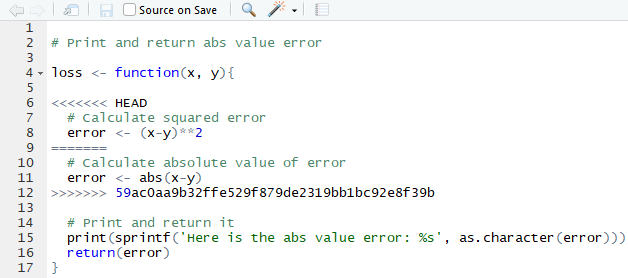
\includegraphics{images/lossConflict.PNG}
\caption{\emph{Conflicted Version of Loss Script}}
\end{figure}

The \texttt{\textless{}\textless{}\textless{}\textless{}} and
\texttt{\textgreater{}\textgreater{}\textgreater{}\textgreater{}} lines
are in the script to signal the beginning and end of a merge conflict,
whereas the \texttt{===} line separates the two different versions. On
the top is Grace's version and on the bottom is Carlos's. To resolve the
merge conflict, Grace should manually select the two lines she prefers
and then delete all of the \texttt{\textless{},\ =,\ \textgreater{}}
symbols to let Git know that the conflict has been resolved. Then, she
can commit and push the file to Git, and she'll be good to go!

Overall: merge conflicts are rather annoying and can be confusing, so
the best way to avoid them is to clearly delineate which programmers
will be working on which sections of which scripts. This will prevent
Git (and you) from getting confused.

\paragraph{Suggested Workflow}\label{suggested-workflow}

There are many ways to use Git, but
\href{https://nvie.com/posts/a-successful-git-branching-model/}{this
article by Vincent Driessen} describes a pretty intuitive and productive
model for Git branching. It's worth reading or skimming the article (it
includes some great graphics), but it basically involves a couple of
core kinds of branches:

\begin{itemize}
\tightlist
\item
  The \textbf{master} branch is only used for new releases of a
  package/software.
\item
  There are \textbf{hotfixes} branches which are used to fix relatively
  important bugs on releases.
\item
  The \textbf{development} branch is the central branch on which most of
  the development happens; i.e.~fixing minor bugs and adding new
  features between releases.
\item
  There are \textbf{feature branches} which are used to develop new
  features between releases, which are periodically updated with the
  development branch.
\item
  Finally, there are \textbf{release branches} which are used
  exclusively to fix bugs pre-release.
\end{itemize}

Here's an illustration of the core model which Driessen made:

\begin{figure}
\centering
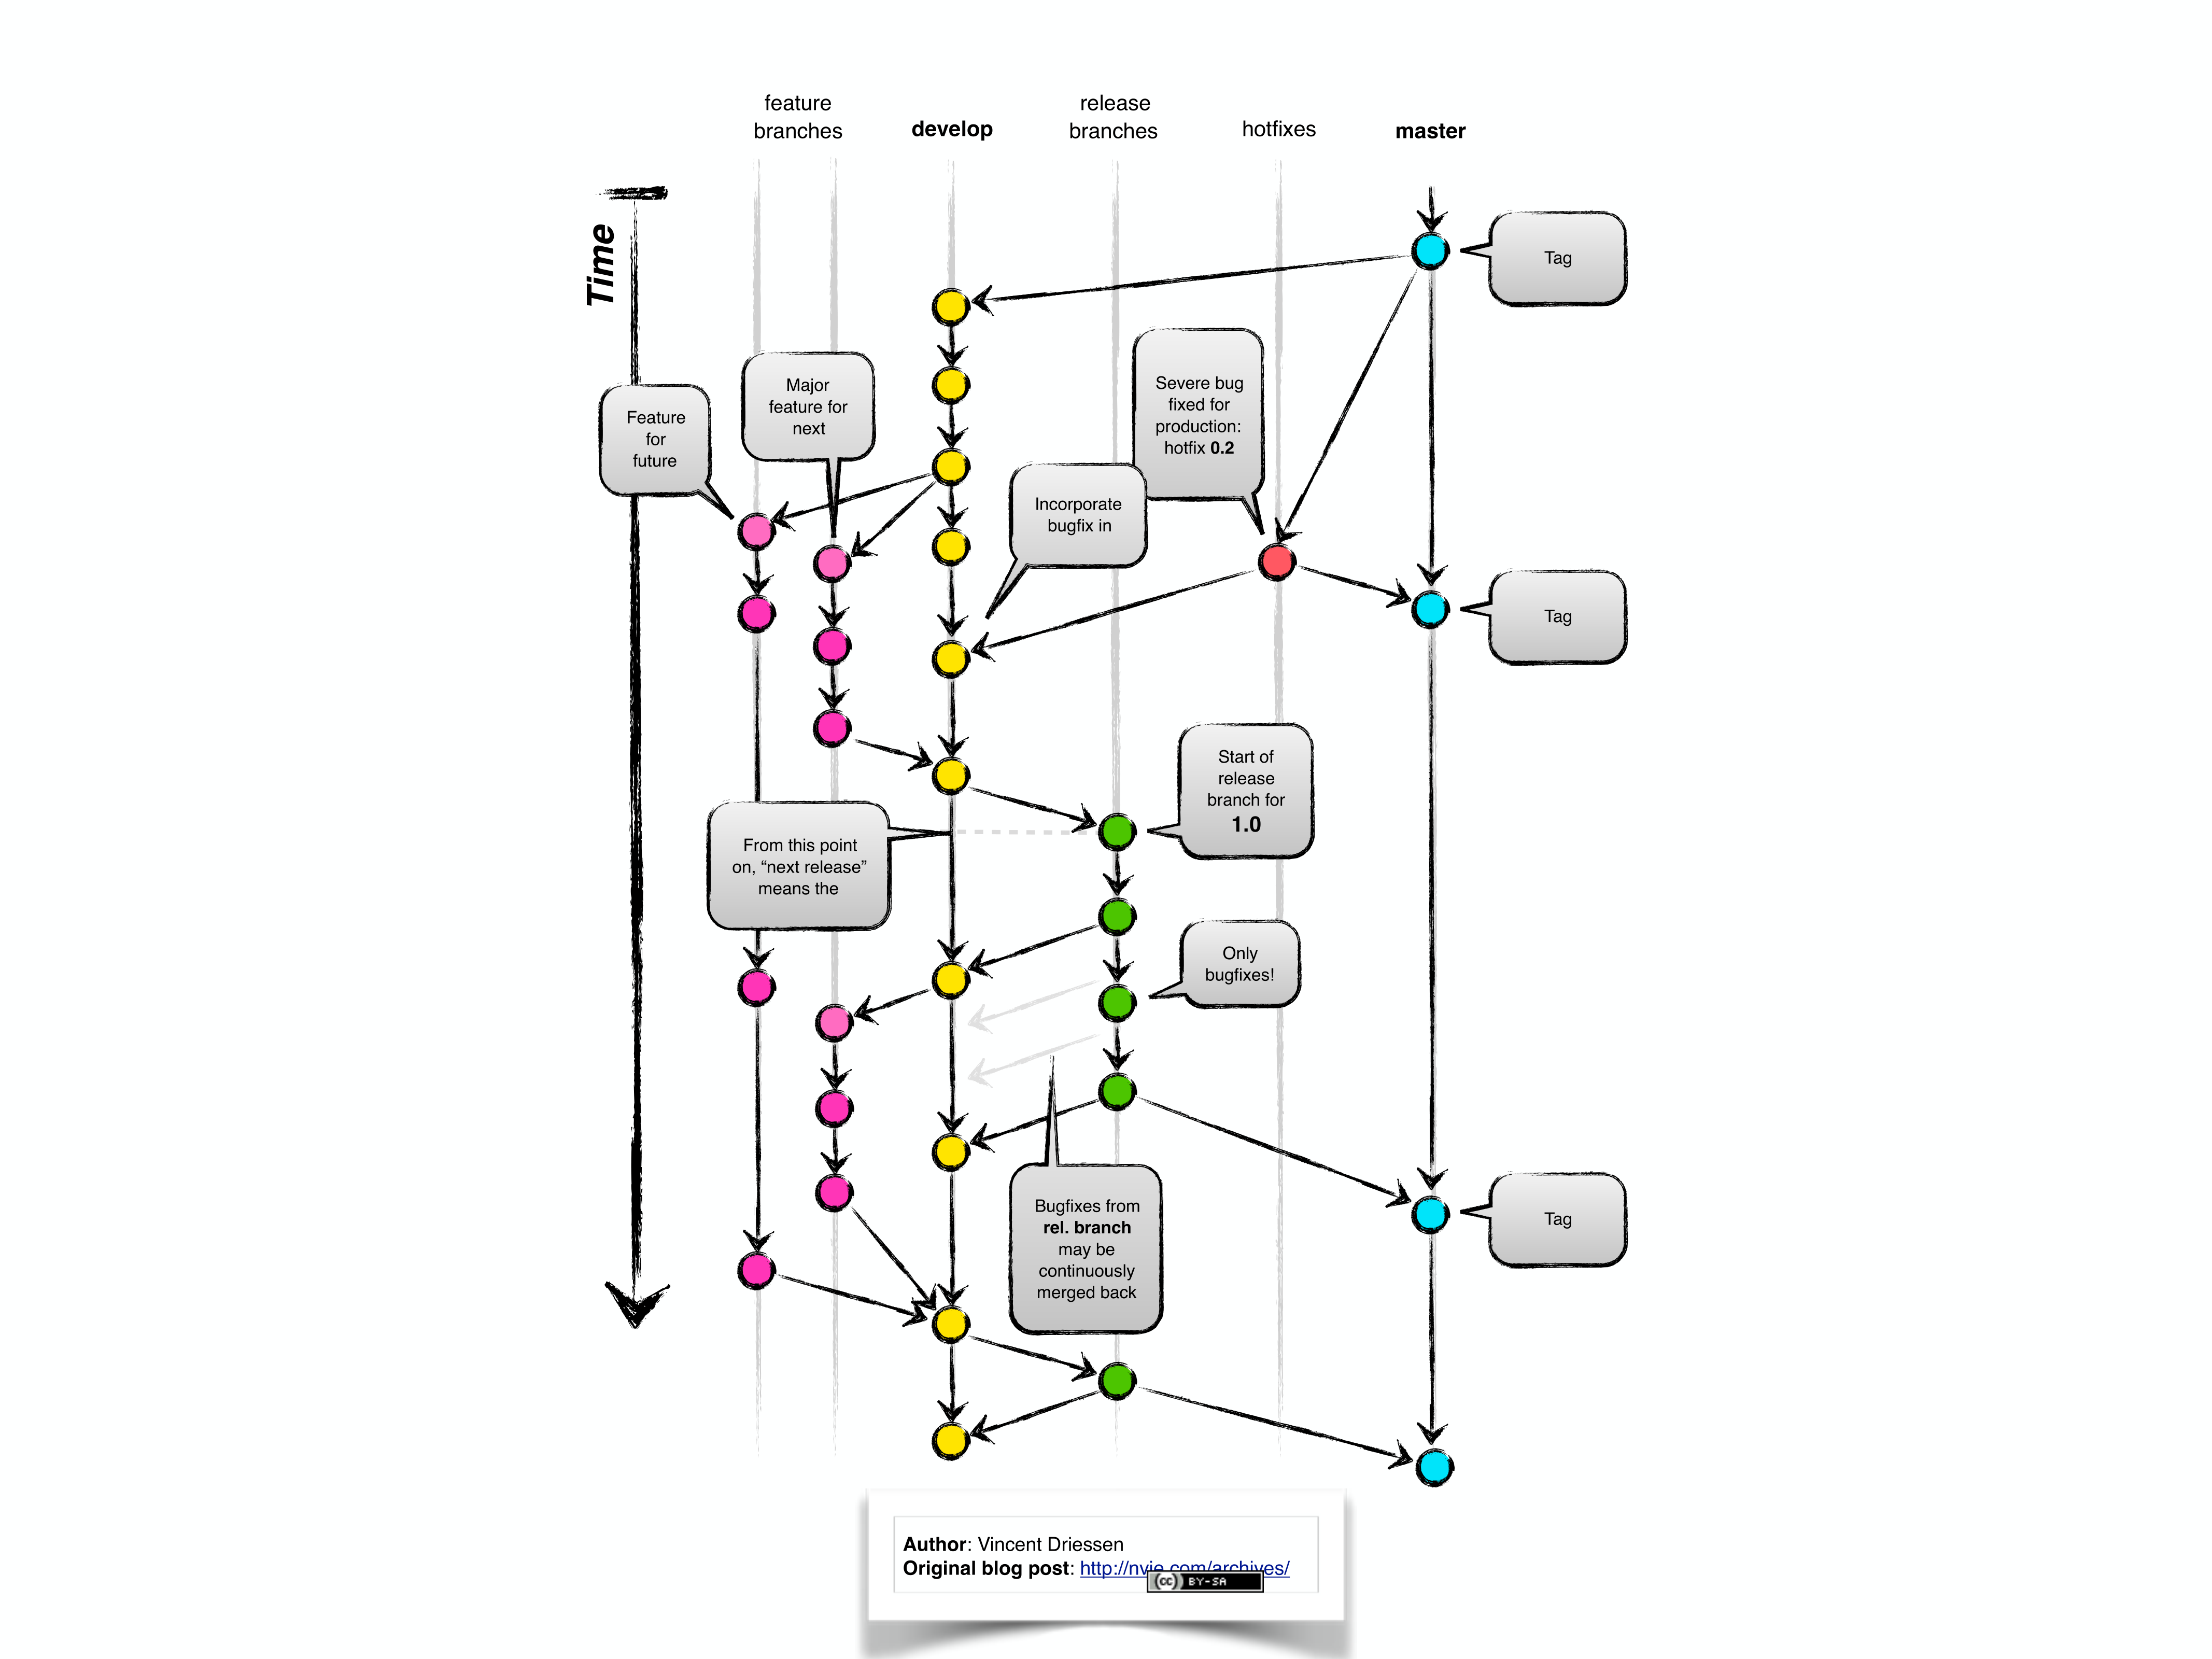
\includegraphics{images/gitflow-model.png}
\caption{}
\end{figure}

\subsection{Tips and Tricks}\label{tips-and-tricks-2}

Git can be confusing, but there are three general rules of thumb you can
follow to figure out any bugs that come up.

\begin{enumerate}
\def\labelenumi{\arabic{enumi}.}
\item
  Git is super smart. If there's a bug and Git is recommending a
  particular way of fixing it, there's a very high chance that Git is
  right.
\item
  Use the \texttt{git\ status} command. After entering
  \texttt{git\ status}, Git will give you a rundown of the status of the
  entire repository.
\item
  If that doesn't work (or you don't understand what is going on), you
  can always copy and paste the error from the command line into Google
  and reference
  \href{https://stackoverflow.com/questions/tagged/git}{stackoverflow}.
  There is a wealth of online help!
\end{enumerate}

Remember that Git almost exclusively \emph{adds information}, meaning
that you can always just go back and restore a previous version - you'll
never lose your work.

Lastly, there are a couple of cheat sheets that you can use to make your
life easier.

\begin{itemize}
\item
  \href{https://stackoverflow.com/questions/tagged/r}{Stackoverflow}
  provides online help for programming in R
\item
  \href{http://kbroman.org/github_tutorial/pages/init.html}{Karl
  Broman's tutorial} runs you through initializing a repository
\item
  \href{https://github.github.com/training-kit/downloads/github-git-cheat-sheet.pdf}{This
  official GitHub cheat sheet} lists all of the general commands you'll
  need
\end{itemize}

\section{Optional: Integrated
Testing}\label{optional-integrated-testing}

\subsection{Why use Integrated Tests?}\label{why-use-integrated-tests}

When working on packages alone, you may not push to GitHub too often.
However, in large projects/packages where many programmers are working
on the same package at once, it's important to ensure each programmer
continuously commits changes to GitHub to make sure all the changes are
compatible with each other. This process of rapid updating of packages
is referred to as \emph{continuous integration}, and it can be very
difficult to manage properly (it is sometimes referred to as
\emph{integration hell}, specifically because developers often waste
lots of hours trying to make code integrate properly). When you commit
changes continuously, it does not guarantee that all the changes will be
compatible. However, if there are compatibility problems in updates, it
does ensure that you'll be able to find those problems more easily,
because each individual change/commit is smaller. For reasons we'll
discuss in a second, continuous integration is a bit easier said than
done. Thankfully, there are two wonderful free continuous integration
services that will make your life a lot easier. If you're using windows,
you'll want to use the service called \emph{Appveyor} - if you're using
Mac or Linux, you'll want to use the service called \emph{Travis CI}.
These services will make continuous integration easy, specifically
because both Appveyor and Travis CI link to GitHub and will run your
build and tests for you on what are called virtual machines in the
cloud.

Maybe the principle of continuous integration makes sense, but why are
continuous integration services useful? Why can't each developer build
packages, run the tests locally, and then only push changes to GitHub if
the tests are successful? There are three answers to this question.

\begin{enumerate}
\def\labelenumi{\arabic{enumi}.}
\tightlist
\item
  For large projects, it often takes a long time to build them. Being
  able to build them on the cloud (using Appveyor/Travis) saves an
  enormous amount of time. (This is especially true for programming
  languages besides R, but it's true for R too!)
\item
  Sometimes there may be global environmental settings on your
  particular computer which change the way the package works and the way
  tests run. Building and testing the package in a ``clean'' environment
  online makes the testing more robust.
\item
  Lastly, CI services offer settings to automatically `deploy' or
  publish successful builds, for example by publishing code for a
  website. These are a bit beyond the scope of this guide, but they are
  documented \href{https://www.appveyor.com/docs/deployment/}{here
  (Appveyor)} and
  \href{https://docs.travis-ci.com/user/deployment/}{here (Travis)}.
\end{enumerate}

\subsection{The integrated testing
workflow}\label{the-integrated-testing-workflow}

It's important to note that Travis/Appveyor do not prevent you from
pushing bad code to a repo - if you break your package and all your
tests fail on Travis/Appveyor, you can still push the broken version to
the master branch on GitHub. As a result, most developer teams use the
following workflow to keep the master branch working at all times.

\begin{enumerate}
\def\labelenumi{\arabic{enumi}.}
\tightlist
\item
  Someone sets up a ``master repo'' with a master branch on GitHub.
\item
  Each developer on the team creates a copy (also called a \emph{fork})
  of the master repo. Thus, each developer has their own repository.
\item
  Each developer makes changes to the project and then pushes those
  changes to their personal fork. After each push, Appveyor or Travis
  builds the package and test it.
\item
  If the Appveyor/Travis builds are successful, the developer will
  likely send a pull request to the master branch of the master repo,
  which will probably be accepted.
\end{enumerate}

This workflow allows each developer to make changes in their own repo
and continuously build them using Travis/Appveyor without potentially
breaking the master repo's copy.

\subsection{Setting up Integrated
Tests}\label{setting-up-integrated-tests}

\textbf{Step 1}: To get started using continuous integration services,
head to the Travis CI (Linux/Mac OS) or AppVeyor (Windows) website. Once
you are on AppVeyor website, click `SIGNUP FOR HOSTED SERVICE'. We
recommend that you create a new AppVeyor account to sign up by signing
into GitHub. At some point, Travis/AppVeyor will ask you to authorize
its connection to GitHub, which you should authorize.

\textbf{Step 2}: Once you authorize the connection, you need to
specifically select which repos you'd like to use Travis/AppVeyor with.
For example (in AppVeyor), upon signing up, you'll see something like
this screen:

\begin{figure}
\centering
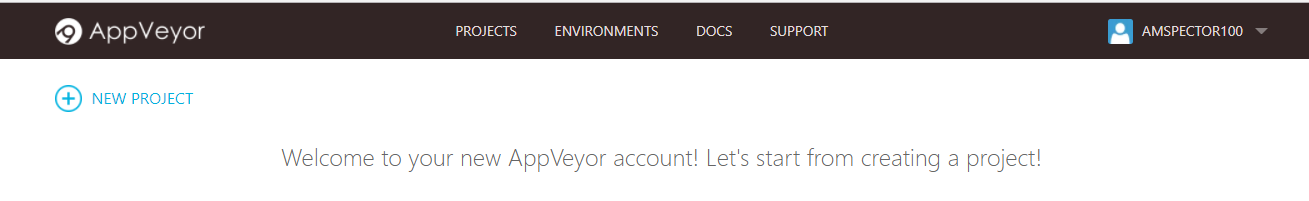
\includegraphics{images/testSS/appveyor1.PNG}
\caption{}
\end{figure}

You should click ``new project'' and then select the specific repo you'd
like to use in combination with Travis/Appveyor by clicking on ``ADD''.
This means that you should at least initialize your project and push it
to GitHub before you start using Travis/Appveyor.

\textbf{Step 3}: Depending on whether you're using Appveyor or Travis,
you should run \texttt{usethis::use\_appveyor()} or
\texttt{usethis::use\_travis()} in the console with your local
repository open. This will create a file named `appveyor.yml' or
`travis.yml' in the root directory of your local repository. These
`.yml' files will tell AppVeyor/Travis what to do. It's actually not too
important to understand everything they do, just because the devtools
template generally works pretty well. However, you occasionally will
have to modify it to suit specific needs. AppVeyor and Travis CI both
have great documentation, linked
\href{https://www.appveyor.com/docs/build-configuration/}{here for
Appveyor} and \href{https://docs.travis-ci.com/user/languages/r/}{here
for Travis}.

(Note - \texttt{usethis} also adds `appveyor.yml' and `travis.yml' to
the .Rbuildignore to reduce clutter in your package.)

\textbf{Step 4: Dependency Issues}: If you're using Travis, it's
important to talk quickly about dependencies in packages. Travis was not
originally designed for R projects, so occasionally it's a bit shaky,
specifically with regard to dependencies in packages (i.e.~Travis will
build your package online, but if your package depends on
\texttt{ggplot2}, then Travis will have to install \texttt{ggplot2}
before building your package). By default, Travis/Appveyor automatically
install anything listed in the dependencies listed in the DESCRIPTION
file for your project. However, occasionally something goes wrong. If
you get error messages that look like Travis did not install all of the
dependencies, it's worth specifying them in the .yml file. You can by
adding a line like the following:

\begin{Shaded}
\begin{Highlighting}[]
\NormalTok{build_script}\OperatorTok{:}
\StringTok{  }\OperatorTok{-}\StringTok{ }\NormalTok{r_packages}\OperatorTok{:}\StringTok{ }\NormalTok{package_name}
\end{Highlighting}
\end{Shaded}

under \emph{build\_script} section in the .yml file (this will install
the package the same way that R installs it when you run
\texttt{install.packages()}). If you'd like to install a package using a
different method (i.e.~from a GitHub version of the package), there are
lots of options listed in the
\href{https://docs.travis-ci.com/user/languages/r/}{R-specific Travis
documentation}. However, it's important to remember that this is
generally NOT necessary - Travis/Appveyor do a pretty good job of
automatically detecting/installing dependencies as long as your
DESCRIPTION file specifies them.

\textbf{Step 5}: If you are working with many other developers on a
single package, you should also add a `.gitattributes' file into the
root of your directory. This is because different operating systems
handle different characters, for example line terminators, slightly
differently. Modern Mac and Unix/Linux systems use
\texttt{\textbackslash{}n} to terminate the end of each line, in what is
called the `line feed' or `LF' system, whereas Windows uses
\texttt{\textbackslash{}r\textbackslash{}n} in the `Carriage Return Line
Feed' or `CRLF' system. The point is that the `.gitattributes' file will
ensure that each developer uses exactly the same line endings, because
you can set the `text' setting which controls the method of writing line
terminators.

The way it works is that the `.gitattribute' file should be a line of
path-patterns followed by specific attributes. These path-patterns (for
a refresher, see the Atlanian guide
\href{https://www.atlassian.com/git/tutorials/saving-changes/gitignore}{here})
are exactly the same path-patterns used in the .gitignore file, just for
a different purpose. For example, one line might be

\begin{Shaded}
\begin{Highlighting}[]
\OperatorTok{*}\StringTok{ }\NormalTok{text=auto}
\end{Highlighting}
\end{Shaded}

where the ``*" refers to all files in the root directory, and the
`text=auto' sets the `text' attribute to auto. Alternatively, you could
write

\begin{Shaded}
\begin{Highlighting}[]
\NormalTok{R}\OperatorTok{/}\ErrorTok{*}\StringTok{ }\NormalTok{text=lf}
\end{Highlighting}
\end{Shaded}

which forces all the scripts directly in the R subdirectory to use the
`lf' line terminator. You can personalize the .gitattributes file if you
like, but you can also just use the sample .gitattributes linked
\href{https://GitHub.com/krlmlr/r-appveyor/blob/master/.gitattributes}{here}.
You can download this file and move it to the root directory of your
package (it must be in the root directory).

The .gitattributes file actually is useful for setting a variety of
other attributes besides line endings, although some of them are a bit
technical. If you're curious to find out more about what the
.gitattributes file can do, the full documentation is linked
\href{https://git-scm.com/docs/gitattributes}{here}.

Once you do all of this, you're set to go! When you push changes to
GitHub, all the new files (.yml, .gitignore, .gitattributes) you created
will be pushed to the remote. By clicking ``NEW BUILD'', Travis/AppVeyor
will automatically build and test the package for you. For example on
Appveyor, if you sign in, you should see something like this:

\begin{figure}
\centering
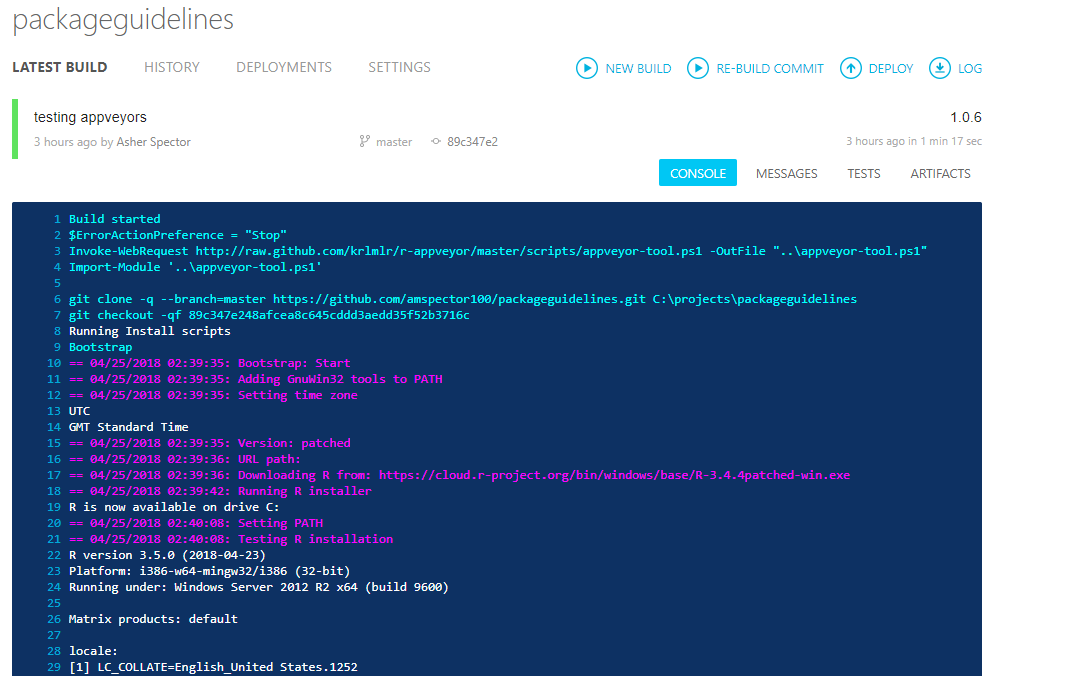
\includegraphics{images/testSS/appveyor2.PNG}
\caption{}
\end{figure}

and if your build succeeded, you'll see a green line at the bottom like
this:

\begin{figure}
\centering
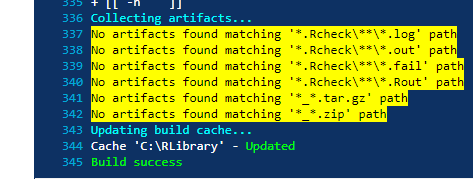
\includegraphics{images/testSS/appveyor3.PNG}
\caption{}
\end{figure}

otherwise you'll see an error. If your build takes a while, that's okay
- you don't need to wait for it to build, because Travis/Appveyor will
email you automatically if the test fails. And that's all there is to
it!

\section{Further reading}\label{further-reading}

If you're interested in learning more about Git and GitHub, you might
want to take a look at the following resources:

\begin{itemize}
\item
  The Software Carpentry Foundation has a great mid level Git tutorial
  \href{https://swcarpentry.GitHub.io/git-novice/}{here}
\item
  Atlassian has some wonderful advanced Git tutorials
  \href{https://www.atlassian.com/git/tutorials/advanced-overview}{here}
\end{itemize}

\chapter{Integrated Development
Environments}\label{integrated-development-environments}

\section{General Suggestions}\label{general-suggestions}

An Integrated Development Environment, or IDE, is simply a piece of
software which aims to make it easier to write and work with packages.
If you're reading this guide, you'll probably spend a decent amount of
time writing packages, so we thought it'd be helpful to review a couple
of different IDEs.

Broadly, there are two kinds of IDEs.

\begin{enumerate}
\def\labelenumi{\arabic{enumi}.}
\tightlist
\item
  Some IDEs are \textbf{language agnostic}, meaning that they support
  any programming language you care to program in. Language-agnostic
  IDEs are nice because (a) if you use one, you won't have to switch
  IDEs every time you use a different programming language, and (b)
  because you can write packages in multiple languages in them.
\item
  On the other hand, some IDEs are \textbf{language specific} in that
  they are built for certain languages. Language specific IDEs can be
  useful because they have a host of speciailized features for their
  specific language.
\end{enumerate}

There are lots of different IDEs available for R users. Common language
agnostic choices include \href{https://atom.io/}{Atom},
\href{https://code.visualstudio.com/}{Visual Studio Code},
\href{https://github.com/jupyterlab}{JupyterLab},
\href{https://www.gnu.org/software/emacs/}{emacs} and
\href{http://aquamacs.org/}{aquamacs}, and even
\href{https://www.sublimetext.com/}{Sublime Text 3}. However, RStudio is
probably the most common and beginner-friendly IDE for R Users, so we'll
focus on RStudio.

\section{RStudio}\label{rstudio}

RStudio is a language-specific IDE built for R, although it does support
plenty of other languages.

\subsection{Why use RStudio?}\label{why-use-rstudio}

RStudio integrates documentation, makes graphics more accessible, and
also combines beautifully with \texttt{devtools} and \texttt{usethis} to
make it easy to write packages. We'll walk through how to set up
RStudio, and then look at two concrete examples: initializing and
building R packages.

\subsubsection{Setting up R}\label{setting-up-r}

Presumably you've already been working with R, but you should make sure
you have a recent enough version of R intalled. To do so, type
\texttt{R.Version()} into the editor you've been working with
previously. It should return an output titled \texttt{version.string},
for example:

\begin{Shaded}
\begin{Highlighting}[]
\KeywordTok{R.Version}\NormalTok{()}
\end{Highlighting}
\end{Shaded}

\begin{verbatim}
## $platform
## [1] "x86_64-pc-linux-gnu"
## 
## $arch
## [1] "x86_64"
## 
## $os
## [1] "linux-gnu"
## 
## $system
## [1] "x86_64, linux-gnu"
## 
## $status
## [1] ""
## 
## $major
## [1] "3"
## 
## $minor
## [1] "6.1"
## 
## $year
## [1] "2017"
## 
## $month
## [1] "01"
## 
## $day
## [1] "27"
## 
## $`svn rev`
## [1] "76783"
## 
## $language
## [1] "R"
## 
## $version.string
## [1] "R version 3.6.1 (2017-01-27)"
## 
## $nickname
## [1] "Action of the Toes"
\end{verbatim}

If the number after the R version string is anything lower than 3.0.1,
you'll have to install a new version of R in order to use R Studio. To
do so, follow the steps below:

\begin{enumerate}
\def\labelenumi{\arabic{enumi}.}
\item
  Go to \url{https://cran.rstudio.com/} and select ``Download R for
  {[}Your Operating System{]}.''
\item
  Click ``base'' and click ``Download R {[}latest version{]} for {[}Your
  Operating System{]}'' at the top of the page.
\item
  You can then let the installer run itself - the default settings
  should be fine for our purposes.
\end{enumerate}

Lastly, updating R on Windows can be a bit tricky. If you use Windows,
you can also use the \texttt{installr} package to quickly update R, as
documented
\href{https://www.r-statistics.com/2015/06/a-step-by-step-screenshots-tutorial-for-upgrading-r-on-windows/}{here}.
However, if you are having trouble installing the \texttt{installr}
package, you can always just follow the instructions above.

\subsubsection{Setting up RStudio}\label{setting-up-rstudio}

To download and set up RStudio, follow the instructions below:

\begin{enumerate}
\def\labelenumi{\arabic{enumi}.}
\item
  Head to \url{https://www.rstudio.com/products/rstudio/download/} and
  click ``download'' for the free RStudio Desktop version
\item
  Download the \emph{installer} for your operating system, not the
  \emph{zip/tarball.} The picture below illustrates what the webpage
  should look like.
\end{enumerate}

\begin{figure}
\centering
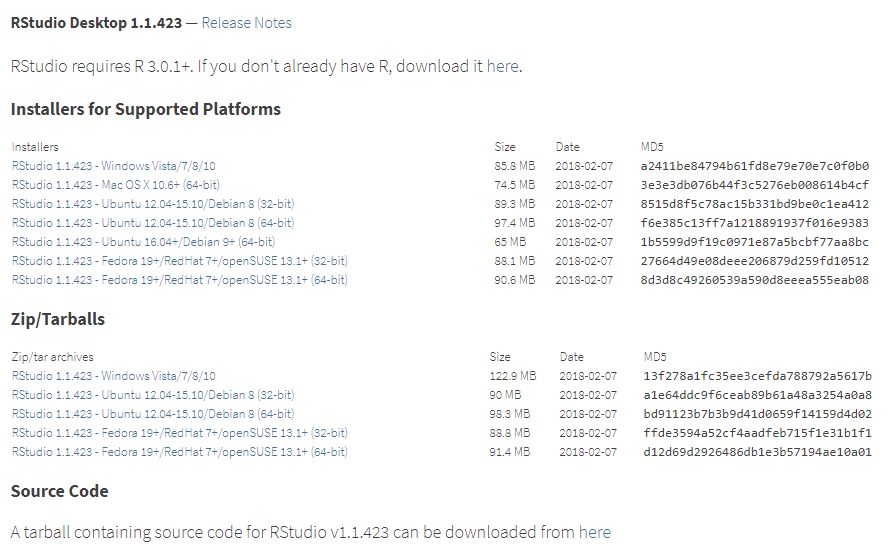
\includegraphics{./images/rstudio.PNG}
\caption{\emph{RStudio Webpage}}
\end{figure}

\begin{enumerate}
\def\labelenumi{\arabic{enumi}.}
\setcounter{enumi}{2}
\tightlist
\item
  Let the installer run - it's fine again to just use the default
  options.
\end{enumerate}

and now you're ready!

\subsection{Getting Started}\label{getting-started}

\subsubsection{Screen Breakdown}\label{screen-breakdown}

RStudio will split your screen into four parts, as shown below. We'll
refer to them as the \emph{script}, the \emph{environment}, the
\emph{shell} or \emph{console}, and the \emph{Viewer.}

\begin{figure}
\centering
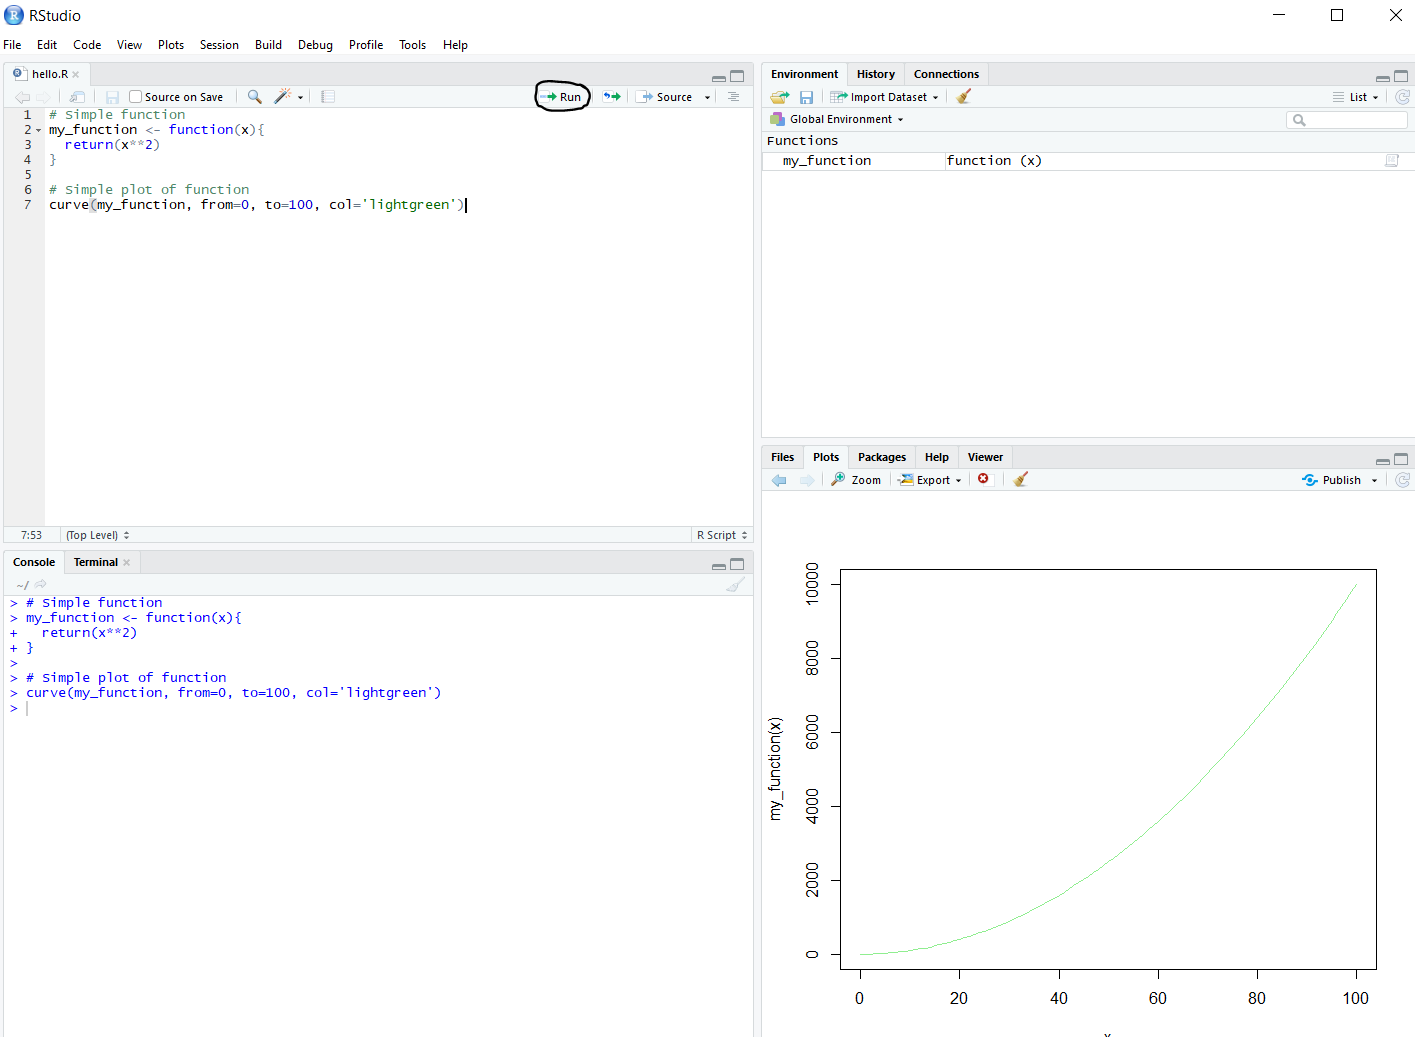
\includegraphics{./images/rstudio2.PNG}
\caption{The RStudio Interface}
\end{figure}

The \emph{script} is in the upper left hand corner of the screen, and
it's where you will do the bulk of your programming. To write an R
script, click File\textgreater{}New File\textgreater{}R Script in the
top left hand corner. You can execute multiple lines of a script (or the
entire thing) at a time by selecting the lines you want to run and
clicking the green ``Run'' button on the right hand side of the script
box or by holding down the command key (MacOS) or control key (Windows)
and pressing return/enter.

The \emph{console} or \emph{shell} is in the lower left hand corner of
the screen. Unlike scripts, which presumably you've worked with before,
shells only run one line of code at a time. However, shells also
remember what you did before. For example, if you download some data
into the shell, you can manipulate it repeatedly without having to
download it again before each manipulation - it will stay in the shell's
memory until you manually remove it.

All scripts that you run will be run through the shell. This means that
you can run a script and manipulate the results directly from the bottom
of the shell, without having to rerun the script each time you want to
manipulate the results. You can also directly access the command prompt
for your computer through the shell by clicking the ``terminal'' option.

Note that any errors thrown by your code will show up in the shell. To
clear the console, hit Ctrl+L.

On the upper right hand corner of the screen, you can see the
\emph{environment} you're working in, which lists all the objects in the
shell's ``memory'' or \emph{namespace.} For example, if you download
some data in a script and then run the script, the data will show up in
the right hand corner of the screen.

On the bottom right hand side is the \emph{Viewer.} Any plots you
generate in R will automatically show up there. Additionally, as we'll
discuss later, documentation of functions and packages will appear in
the right hand corner. You can also use it to see the file structure of
your working directory and the packages you're using by clicking
``files'' or ``packages.''

\subsection{Ex: Initializing Packages}\label{ex-initializing-packages}

RStudio makes it easy to create packages. To start, click
File\textgreater{}New Project. Then, click ``New Directory'' when you
see the screen below:

\begin{figure}
\centering
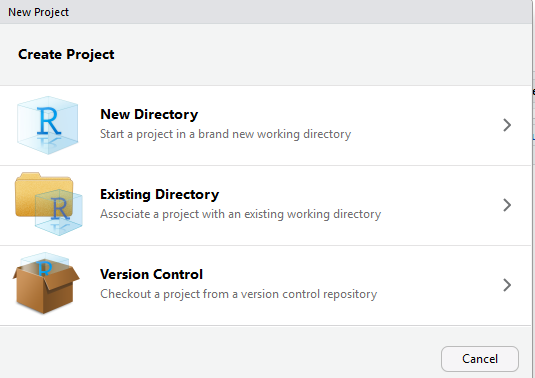
\includegraphics{images/packageSS/createproj1.PNG}
\caption{}
\end{figure}

Then click ``R Package'' when you see the screen below:

\begin{figure}
\centering
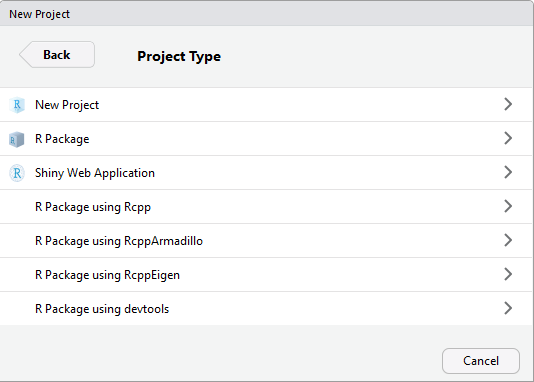
\includegraphics{images/packageSS/createproj2.PNG}
\caption{}
\end{figure}

Lastly, name your package. Your name should be something short and
descriptive. Since we'll be walking through a development example, we'll
title our new package \texttt{devex}.

\begin{figure}
\centering
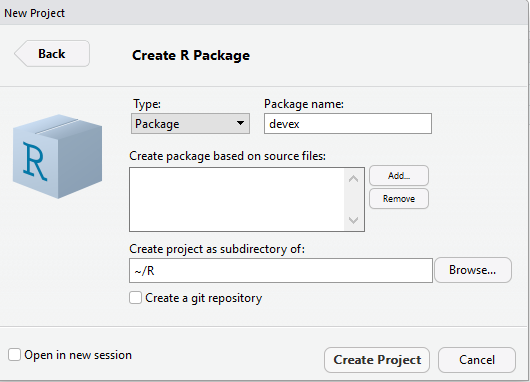
\includegraphics{images/packageSS/createproj3.PNG}
\caption{}
\end{figure}

Once you've created your package, your RStudio should look something
like this. It should come preloaded with a ``Hello World'' script which
includes a handy function that prints ``Hello world.''

\begin{figure}
\centering
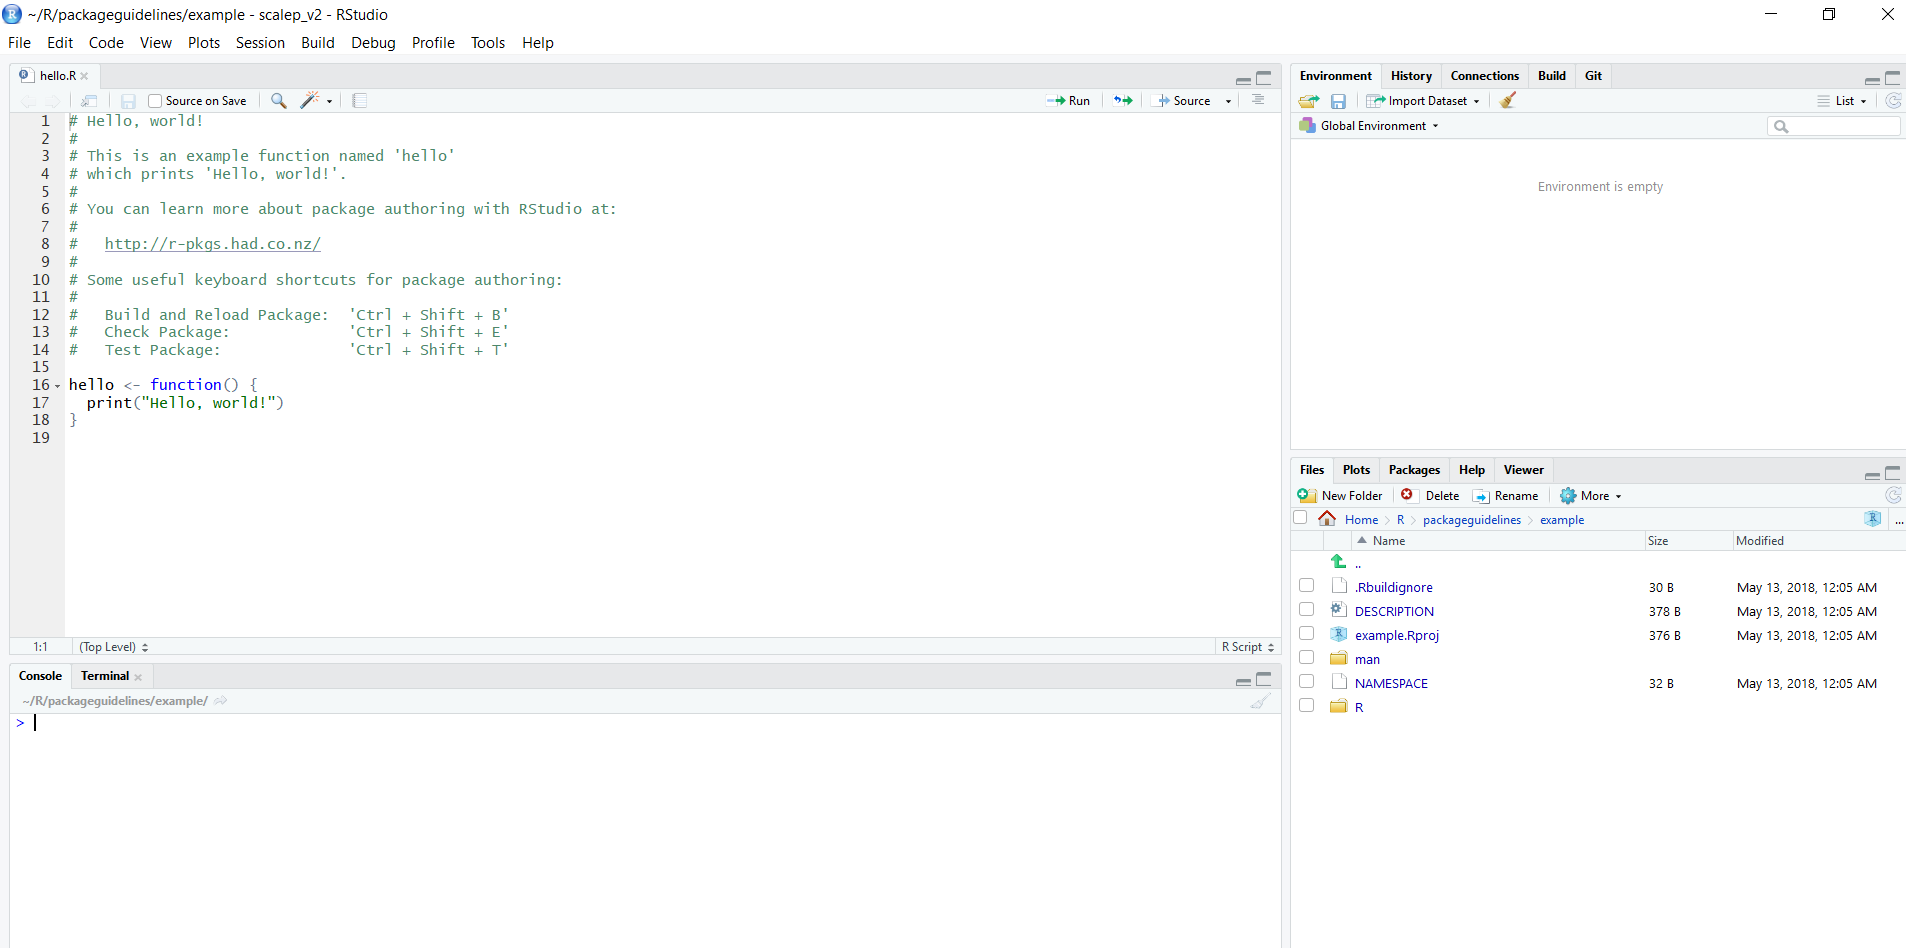
\includegraphics{images/packageSS/projectinit.PNG}
\caption{}
\end{figure}

Everything should look mostly the same as normal except for the
``Files'' tab on the bottom right, which should include an ``.Rproj''
file, a ``DESCRIPTION'' file, a ``NAMESPACE'' file, and a folder titled
``R.'' You should start by checking the little boxes next to the
``NAMESPACE'' file and the ``Hello.R'' R script inside the R file and
clicking ``delete'' above them, just because we will have Roxygen2
automatically generate the namespace, and because presumably your
package doesn't need a ``Hello World'' function.

You should also go to ``Tools \textgreater{} Project Options'' and
select the following options, which will help you generate documentation
using roxygen2. This requires ``roxygen2'' package to be loaded into the
search path first to have the ``Generate documentation with Roxygen''
option displayed.

\begin{figure}
\centering
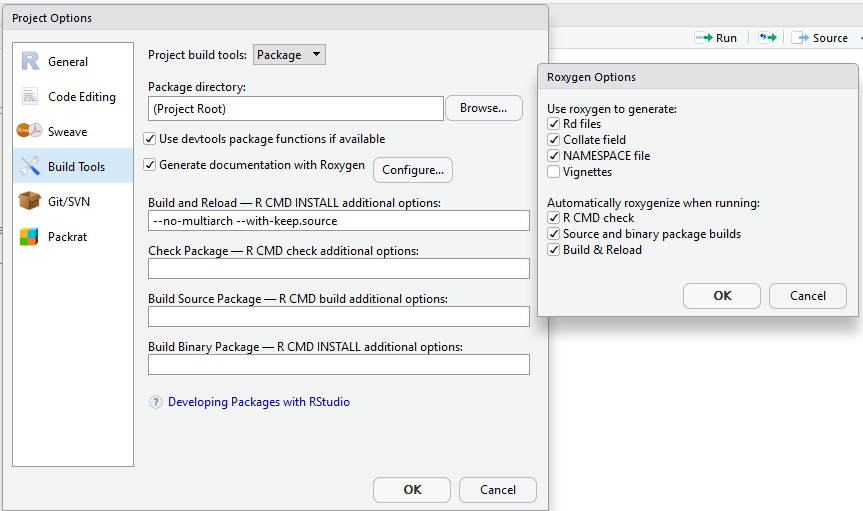
\includegraphics{images/packageSS/userox.PNG}
\caption{}
\end{figure}

\subsection{Ex: Building Packages}\label{ex-building-packages}

RStudio will build your package a little bit more conveniently than the
\texttt{devtools::build()} function will. Whereas the
\texttt{devtools::build()} function, without extra arguments, will
simply bundle your package into one file, building your package from
RStudio will actually install it into your R library, allowing you to
easily use the finished version.

The way to do this is to go to Build \textgreater{} Install and Restart,
and then RStudio will build your package, restart, and load your package
into R (using the \texttt{library()} command). Then, you can use and/or
play with your package!

(If you don't see any options under Build, you probably need to open
your .Rproj file in the ``file'' section of RStudio. Upon doing this,
RStudio should restart briefly and then you will see more Build options.
Note, the .Rproj file may not exist if you created the package with
\texttt{usethis} outside of RStudio).

\chapter{Resources}\label{resources}

\section{General}\label{general}

\begin{itemize}
\tightlist
\item
  \href{https://www.rstudio.com/resources/cheatsheets/}{This link}
  contains a number of truly fantastic cheat sheets, documenting
  everything from RStudio itself to data visualization and machine
  learning.
\item
  To read more about using R, \href{http://adv-r.had.co.nz/}{take a look
  at the following website, built by Chapman and Hall}
\item
  As always, it's worth referencing
  \href{https://stackoverflow.com/questions/tagged/r/}{stackoverflow} if
  you're ever confused. 
\end{itemize}

\section{Package Development}\label{package-development-1}

\begin{itemize}
\tightlist
\item
  There's a wonderful cheat sheet for package development linked
  \href{https://www.rstudio.com/wp-content/uploads/2015/06/devtools-cheatsheet.pdf}{here}.
  This also describes a lot of key components of the testthat package.
\item
  If you are looking for a very simple example of a package, the
  \href{https://github.com/IQSS/Rbuild/tree/master/devex}{devex package}
  can be found here. If you're having trouble understanding the workflow
  for package development, it's worth looking through the \texttt{devex}
  package and making sure you understand all its components. Better yet,
  you can practice using \texttt{roxygen2} and \texttt{devtools} by
  creating a very small/useless package (2-3 simple functions)
\item
  It can sometimes be instructive to look through the
  \href{https://www.rdocumentation.org/packages/devtools/versions/1.13.3/source}{source
  code} and
  \href{https://www.rdocumentation.org/packages/devtools/versions/1.13.3}{documentation}
  for \texttt{devtools}.
\end{itemize}

Additionally, as you build larger and more complex packages, you might
need a deeper understanding of package structure. For a slightly more
in-depth explanation of package development, you'll want to reference
Hadley Wickham's \href{http://r-pkgs.had.co.nz/}{R Packages}. For a
serious dive into package mechanics, you should consult the official
\href{https://cran.r-project.org/doc/manuals/R-exts.html\#Creating-R-packages}{R
Extensions Manual}, which is published by CRAN. However, at least for
mid-sized packages, this guide probably has given you most of what you
need to know.

\section{Version Control}\label{version-control-1}

\begin{itemize}
\tightlist
\item
  \href{https://github.github.com/training-kit/downloads/github-git-cheat-sheet.pdf}{The
  official GitHub cheat sheet} lists all of the general commands you'll
  need
\item
  \href{http://kbroman.org/github_tutorial/pages/init.html}{Karl
  Broman's tutorial} runs you through initializing a repository
\item
  Atlassian's table of the .gitignore syntactical rules is listed
  \href{https://www.atlassian.com/git/tutorials/gitignore}{here}.
\item
  Here are the links to the build configuration docs for
  \href{https://www.appveyor.com/docs/build-configuration/}{Appveyor}
  and \href{https://docs.travis-ci.com/user/languages/r/}{Travis}.
\end{itemize}

If you're interested in reading more:

\begin{itemize}
\tightlist
\item
  The Software Carpentry Foundation has a great mid level Git tutorial
  \href{https://swcarpentry.GitHub.io/git-novice/}{here}
\item
  Atlassian has some wonderful advanced Git tutorials
  \href{https://www.atlassian.com/git/tutorials/advanced-overview}{here}
\end{itemize}

\section{IDEs}\label{ides}

\begin{itemize}
\tightlist
\item
  \href{https://www.theanalysisfactor.com/the-advantages-of-rstudio/}{This
  page} lists some more of RStudio's advantages.
\end{itemize}


\end{document}
